\chapter{Tinjauan Pustaka dan Dasar Teori}
Bab ini akan membahas tinjauan pustaka yang mencakup penelitian-penelitian sebelumnya sebagai referensi untuk melaksanakan tugas akhir. Selain itu, akan dijelaskan tentang teori-teori yang menjadi dasar dalam pembuatan aplikasi tugas akhir.
\section{Tinjauan Pustaka}
% ================================= Penelitian Designing Gamification for Programming Learning Applications =================================
Gamifikasi telah terbukti menjadi strategi populer yang diyakini efektif dalam meningkatkan minat dan motivasi belajar \cite{EnjoyLearningLikeGaming}. 
Berdasarkan beberapa studi yang ada, pengimplementasian gamifikasi yang tepat akan meningkatkan ketertarikan dan motivasi murid dalam proses pembelajaran.
Salah satu studi yang dilakukan pada tahun 2022 oleh Evan Pradanika, Yani Widyani, dan Yanti Rusmawati dengan judul \textit{"Designing Gamification for Programming Learning Applications"} \cite{GamificationInProgLang} membahas mengenai penerapan gamifikasi
dalam sebuah pembelajaran pemrograman. Studi tersebut menerangkan sebuah perancangan desain sistem menggunakan pendekatan \textit{Activity-centered Design} dimana perancangan ini berfokus pada aktivitas utama sebuah pembelajaran\cite{GamificationInProgLang}. 
Implementasi gamifikasi pada penelitian ini berpedoman pada hubungan antara jenis-jenis pengetahuan atau \textit{Type of Knowledge} yang memiliki elemen gamifikasinya masing masing\cite{kapp2012gamification}.
Hubungan ini dijelaskan dalam buku yang ditulis oleh Karl M. Kapp yang berjudul \textit{"The Gamification of Learning and Instruction : Game-based method and strategies for training and education"}\cite{kapp2012gamification}.
Proses pengembangan desain gamifikasi dalam penelitian ini didasari dengan kategori pembelajarannya sendiri yaitu ilmu pemrograman yang dikategorikan sebagai \textit{declarative knowledge}.
Dengan mengevaluasi aplikasi pembelajaran pemrograman yang sudah ada di \textit{Play Store}, Evan Pradanika dan teman-temannya merumuskan desain tersebut berdasarkan kebutuhan user, dan aktivitas pemrogramannya sendiri \cite{GamificationInProgLang}.
Sehingga, elemen gamifikasi yang digunakan dalam penelitian ini diantaranya ada
\textit{Trivia} yang diterapkan dalam latihan-latihan dalam bentuk jawaban singkat dan pilihan ganda,
\textit{Matching} diterapkan dalam latihan-latihan dalam bentuk seret dan lepas,
\textit{Challenges} diterapkan dalam bentuk prestasi yang dapat diperoleh oleh pengguna \cite{GamificationInProgLang}.
Keluaran dari penelitian ini ialah sebuah \textit{High-fidelity prototype} (gambar \ref*{fig:High-fidelity prototype Evan}) yang kemudian diujikan dan dievaluasi menggunakan \textit{Usability Testing} dan \textit{User Experience Goals} untuk mengukur perfroma interaktif produk terhadap penggunanya.
\textit{Usability Testing} yang dilakukan berupa \textit{Completion Rate} untuk mengukur efektivitas, \textit{System Usability Scale (SUS)} untuk mengukur kebergunaan,
\textit{Single Ease Question (SEQ)} untuk mengukur tingkat kesulitan dari aktivitas yang diberikan, \textit{Intrinsic Motivation Inventory (IMI)} yang merupakan instrumentasi untuk mengukur motivasi,
dan \textit{User Engagement Scale-Short Form (UES-SF)} untuk mengukur keterlibatan \cite{GamificationInProgLang}.
% Untuk konteks pembelajaran pemrograman, pemrograman senriri dapat dikategorikan sebagai pengetahuan deklaratif karena memungkinkan pembuatan variabel dengan tipe yang telah ditentukan oleh bahasa pemrograman. 
% Selain itu, pemrograman juga termasuk ke dalam pengetahuan prosedural karena melibatkan urutan eksekusi instruksi dalam sebuah program. 
% Selanjutnya, pemrograman juga termasuk pengetahuan konseptual karena memiliki beberapa konstruksi yang dapat digunakan, seperti if-then-else dan loop, yang merupakan konsep asli dari bahasa pemrograman itu sendiri.
% \newpage

\begin{figure}[H]
	\centering
	\begin{subfigure}[b]{0.4\textwidth}
		\centering
	  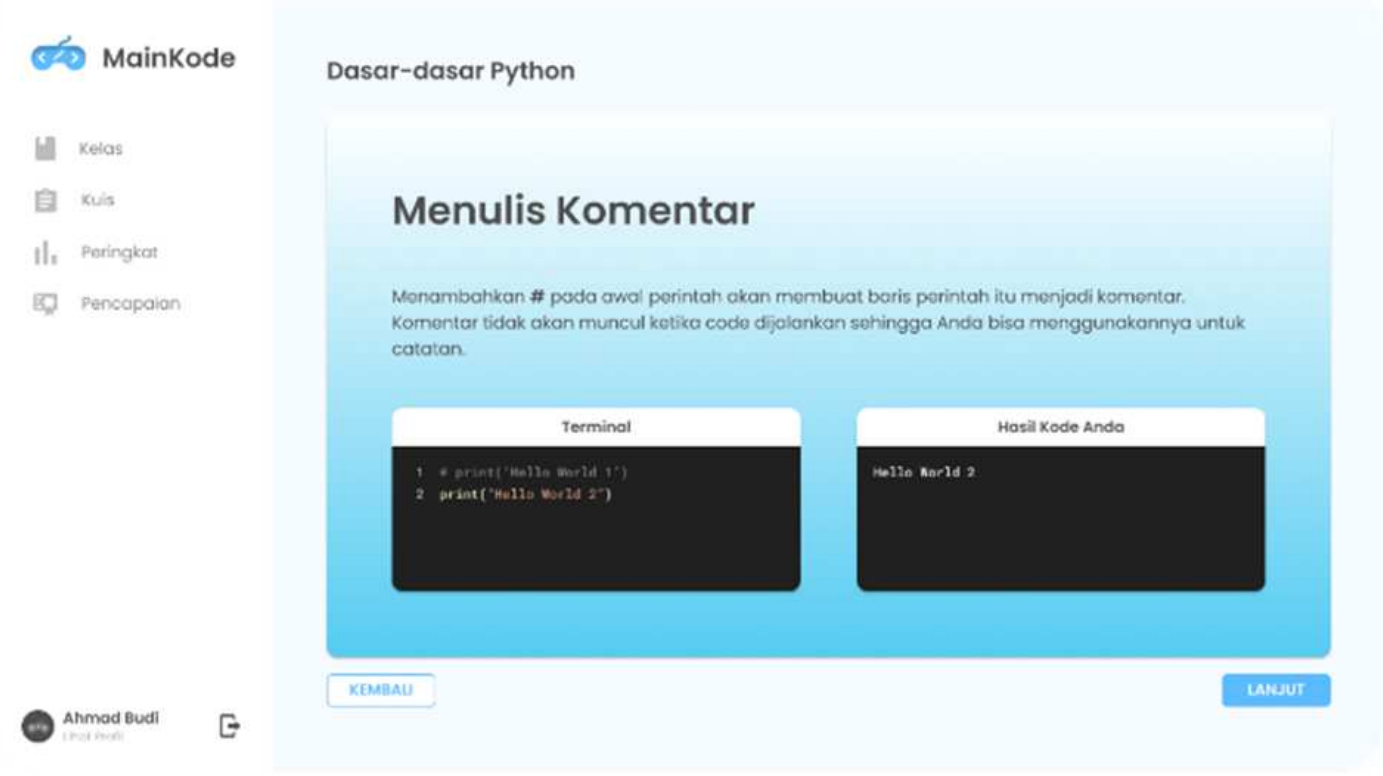
\includegraphics[width=\linewidth]{contents/chapter-2/images/Evan-a1.png}
	  \caption{\textit{Class topic page}}
	  \label{fig:sub1-a1}
	\end{subfigure}
	\begin{subfigure}[b]{0.4\textwidth}
	\centering
	  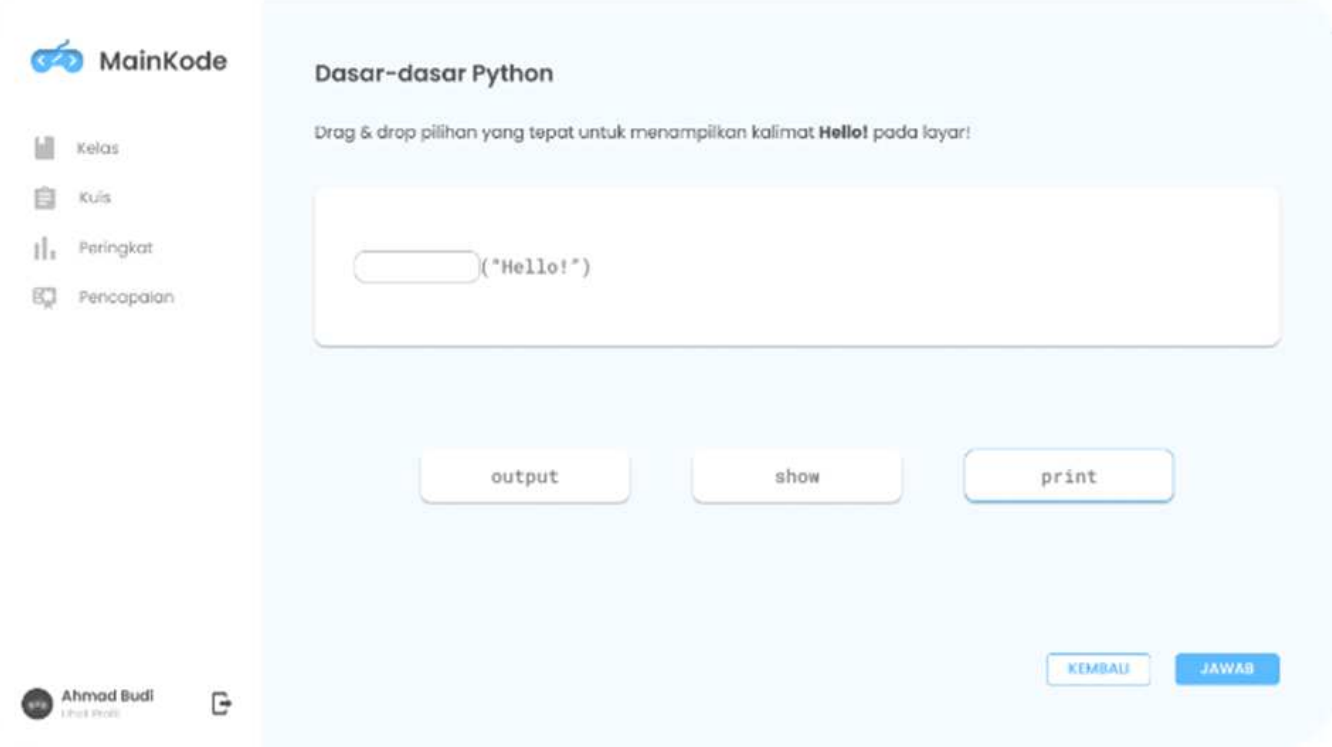
\includegraphics[width=\linewidth]{contents/chapter-2/images/Evan-a2.png}
	  \caption{\textit{Gamified exercise page}}
	  \label{fig:sub2-a2}
	\end{subfigure}
	\hfill
	\begin{subfigure}[b]{0.4\textwidth}
		\centering
		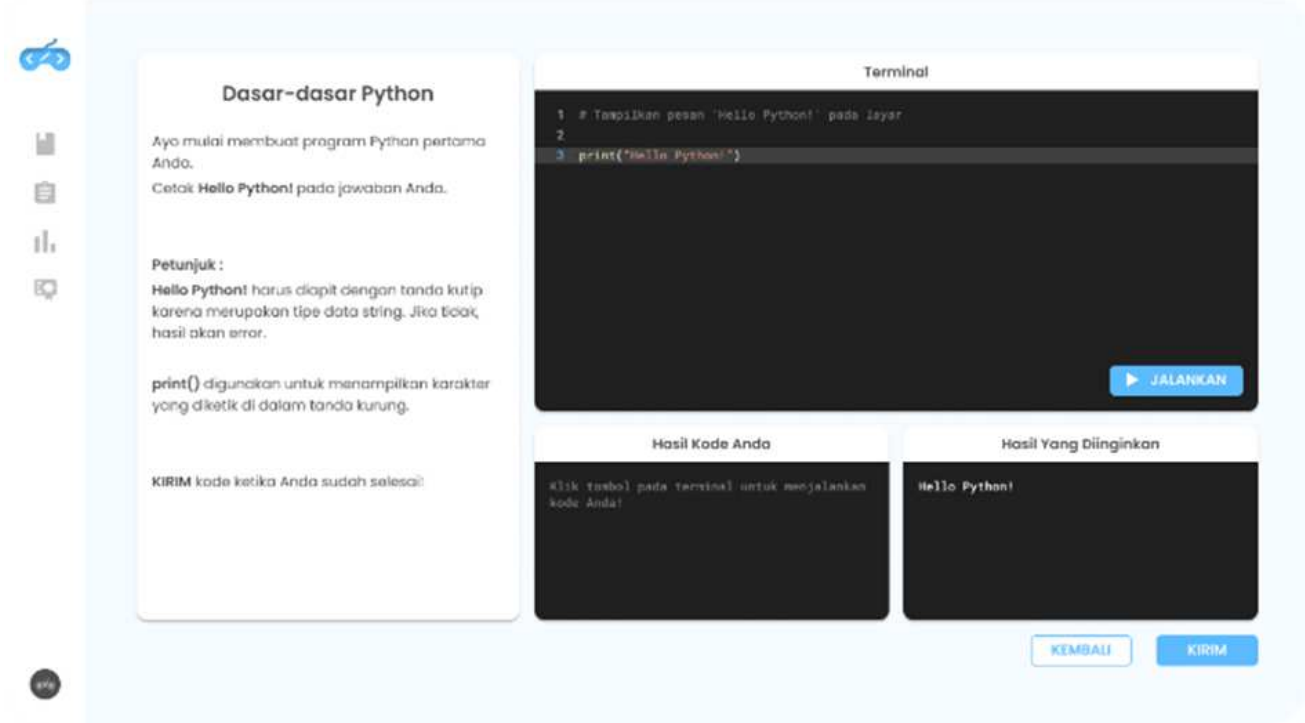
\includegraphics[width=\linewidth]{contents/chapter-2/images/Evan-a3.png}
		\caption{\textit{Terminal exercise page}}
		\label{fig:sub3-a3}
	\end{subfigure}  
	\begin{subfigure}[b]{0.4\textwidth}
		\centering
		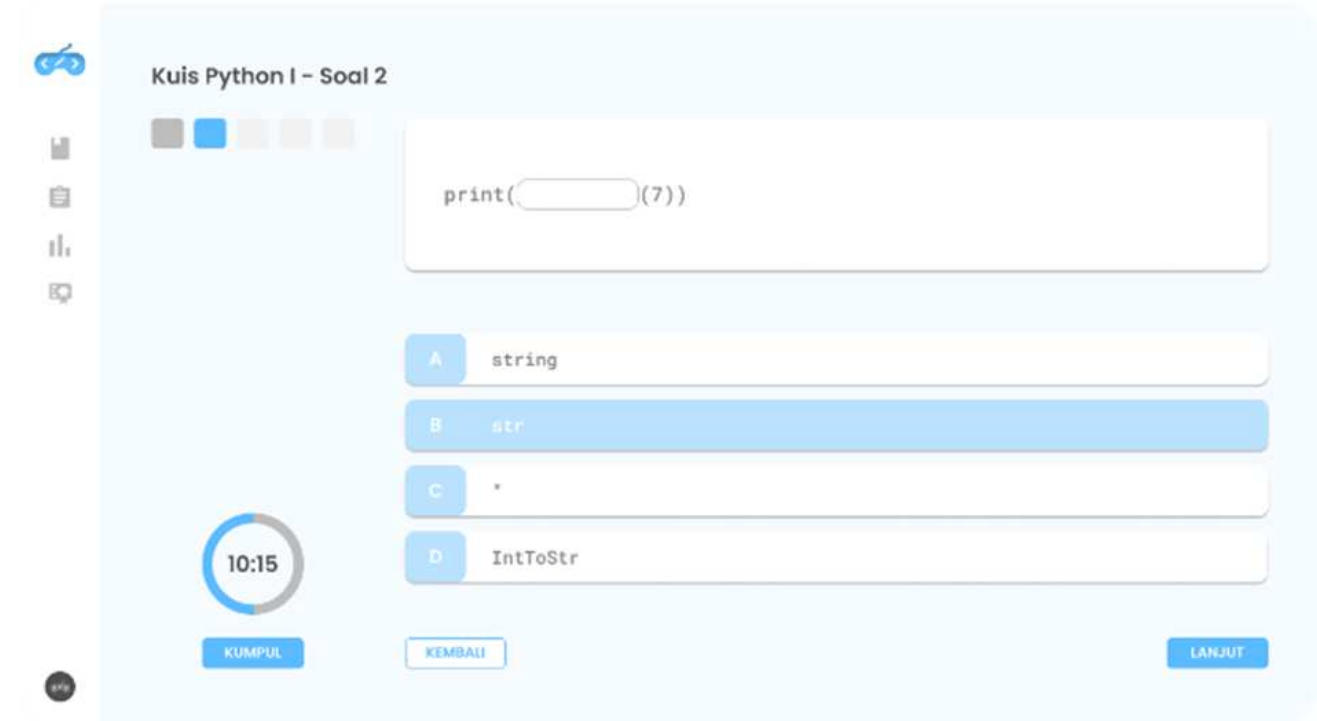
\includegraphics[width=\linewidth]{contents/chapter-2/images/Evan-a4.png}
		\caption{\textit{Quiz page}}
		\label{fig:sub4-a4}
	\end{subfigure} 
	\begin{subfigure}[b]{0.4\textwidth}
		\centering
		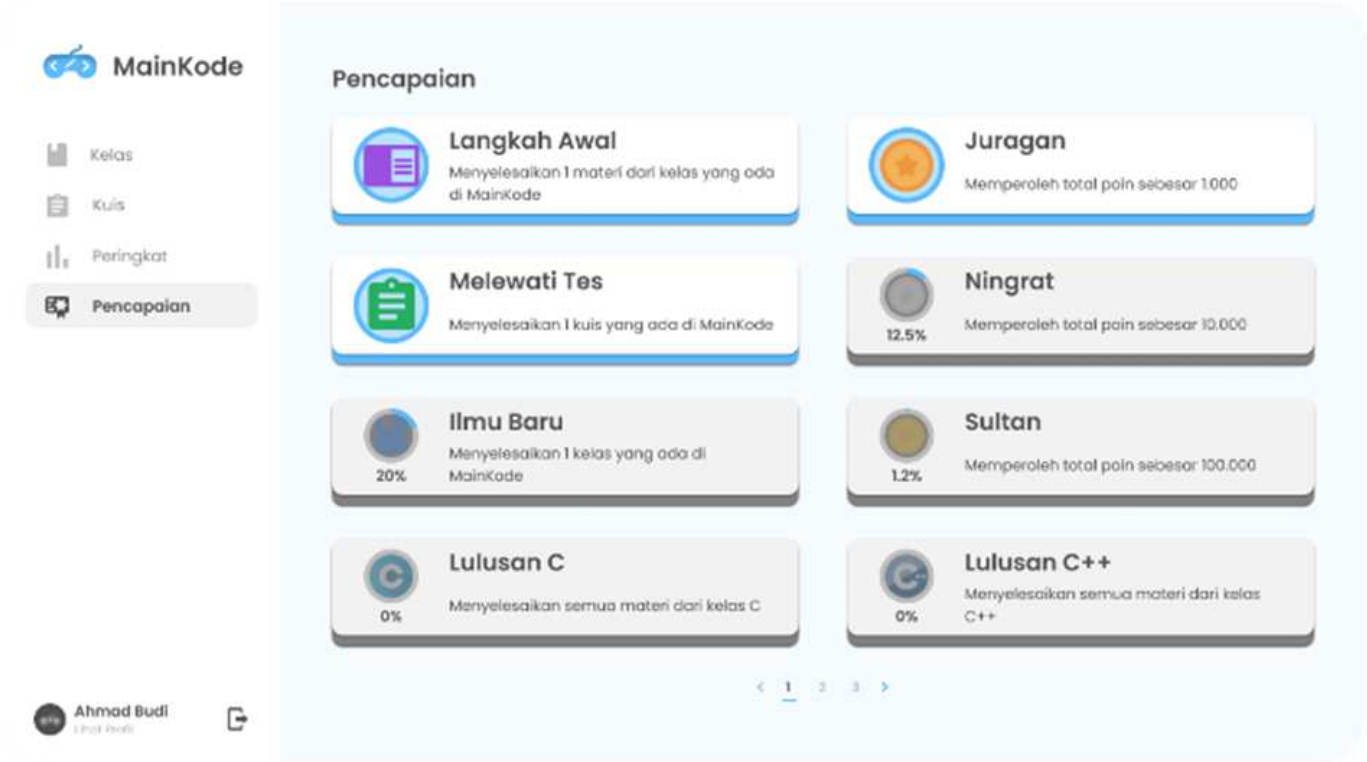
\includegraphics[width=\linewidth]{contents/chapter-2/images/Evan-a5.png}
		\caption{\textit{Achievement page}}
		\label{fig:sub5-a5}
	\end{subfigure} 
	\caption{\textit{High-fidelity prototype} aplikasi pembelajaran pemrograman \cite{GamificationInProgLang}}
	\label{fig:High-fidelity prototype Evan}
  \end{figure}
Ada juga penelitian yang dilakukan pada tahun 2021 oleh Bernadeta Ratna P. S. dan rekan-rekannya mengenai pengembangan desain gamifikasi ini.
Penelitian tersebut memaparkan mengenai pengembangan gamifikasi untuk sebuah media pembelajaran anatomi yang berjudul \textit{"Design of Gamification for Anatomy Learning Media"}\cite{AnatomyGamification}.
Sama halnya dengan penelitian sebelumnya, penelitian ini memiliki tujuan untuk meningkatkan motivasi dan keterlibatan pengguna dalam memahami anatomi tubuh manusia.
Proses pengembangan desain gamifikasi pada penelitian ini menggunakan sebuah \textit{framework game design} yang dinamai \textit{"Elemental Tetrad"}\cite{AnatomyGamification}.
\textit{Framework} tersebut memodelkan gamifikasi dalam 4 bentuk, yakni \textit{Mechanics}, \textit{Aesthetics}, \textit{Story} atau \textit{Dynamics}, dan \textit{Technology}\cite{marisa2020gamifikasi}.
Masing masing elemen desain tersebut kemudian dikembangkan berdasarkan konteks pembelajaran yang akan dipelajari, dalam penelitian ini yaitu pembelajaran anatomi manusia.
\textit{Game Mechanics} dalam penelitiannya terdiri dari \textit{game mode}, \textit{parts}, \textit{points} dan \textit{reward}. 
Untuk elemen \textit{Aesthetics} terdiri dari \textit{ User Interface} dan \textit{User Experience}, \textit{Art}, \textit{Unlocking Parts}, dan \textit{Challenges}.
Untuk \textit{Story}, akan mengikuti alur pembelajaran yang dibagi menjadi 3 bagian, yaitu materi, praktikum, dan kuis\cite{AnatomyGamification}.
Untuk elemen terakhir yaitu teknologi yang digunakan dalam penelitian ini. Penelitian ini menggunakan \textit{Smartphone} dan 3D model dari kerangka manusia \cite{AnatomyGamification}.
Hasil dari penelitianini berupa sebuah aplikasi \textit{Smartphone} yang dapat di-\textit{install} pada sistem operasi \textit{Android}.
Tampilan aplikasi ini dilampirkan pada gambar \ref*{fig:interface pembelajaran anatomi}.
Berbeda dengan penelitian sebelumnya, pada penelitian ini tidak dilakukan pengujian \textit{Usability} dan \textit{User Experience}.
% \newpage
\begin{figure}[H]
	\centering
	\begin{subfigure}[b]{0.4\textwidth}
		\centering
	  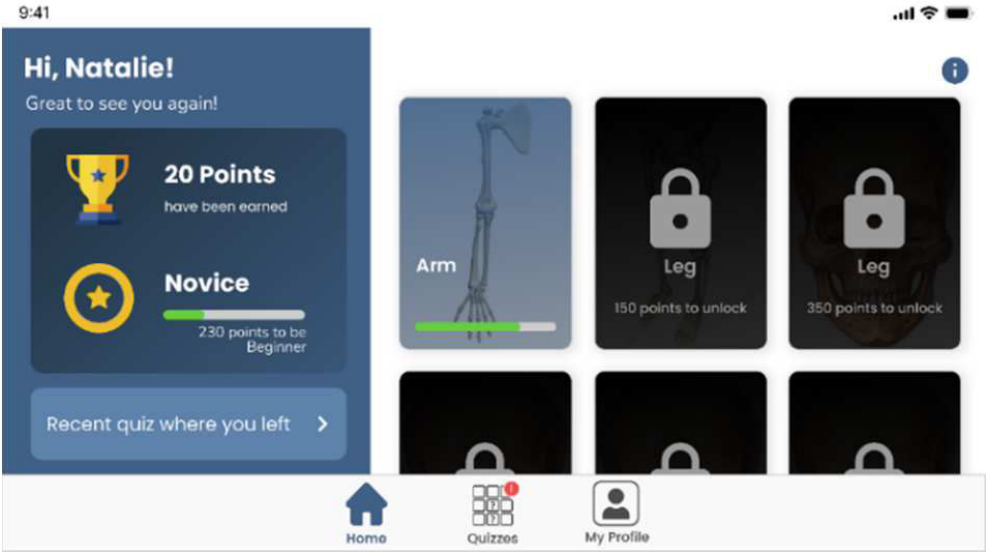
\includegraphics[width=\linewidth]{contents/chapter-2/images/Deta-a1.png}
	  \caption{\textit{Interface design home menu}}
	  \label{fig:sub-deta-a1}
	\end{subfigure}
	\begin{subfigure}[b]{0.4\textwidth}
	\centering
	  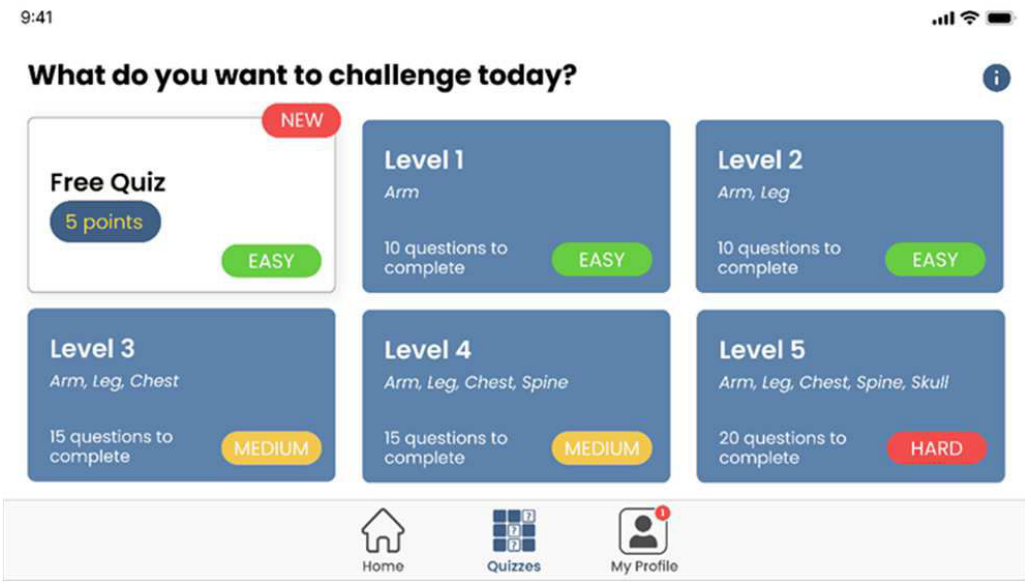
\includegraphics[width=\linewidth]{contents/chapter-2/images/Deta-a2.png}
	  \caption{\textit{Interface design quiz menu }}
	  \label{fig:sub-deta-a2}
	\end{subfigure}
	\hfill
	\begin{subfigure}[b]{0.4\textwidth}
		\centering
		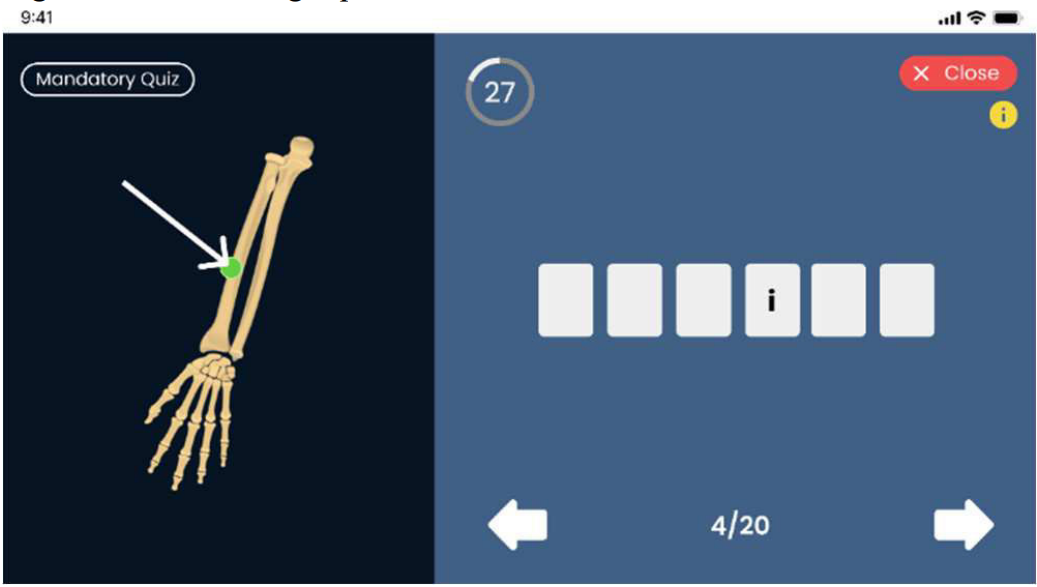
\includegraphics[width=\linewidth]{contents/chapter-2/images/Deta-a3.png}
		\caption{\textit{Interface design mandatory quiz}}
		\label{fig:sub-deta-a3}
	\end{subfigure}  
	\caption{Tampilam aplikasi pembelajaran anatomi \cite{AnatomyGamification}}
	\label{fig:interface pembelajaran anatomi}
  \end{figure}

Adaptasi gamifikasi pada sebuah media pembelajaran juga dijelasakan pada penelitian yang dilakukan oleh Andre Julian Irawan, Fenina Adline Twince Tobing, dan Eunike Endariahna Surbakti
dengan judul \textit{"Implementation of Gamification Octalysis Method at Design and Build a React Native Framework Learning Application"}\cite{OctalysisFrameworkAndre}.
Dalam penelitian ini, proses gamifikasi menggunakan kerangka kerja \textit{Octalysis} atau \textit{Octalysis Gamification Framework} untuk mengembangan sebuah aplikasi pembelajaran yang mempelajari \textit{React Native Framework}.
Kerangka kerja ini meruapakan sebuah kerangka kerja gamifikasi yang dikembangakan oleh Yu-Kai Chou, seorang ahli gamifikasi terkemuka\cite{marisa2020gamifikasi}.
Metode \textit{Octalysis} memiliki delapan inti motivasi yang berfokus pada perilaku manusia, seperti \textit{meaning}, \textit{accomplishment}, \textit{empowerment}, \textit{ownership}, \textit{social influence}, \textit{scarcity}, \textit{unpredictability}, dan \textit{avoidance}\cite{marisa2020gamifikasi}.

\begin{figure}[H]
	\centering
	\begin{subfigure}[b]{0.4\textwidth}
		\centering
	  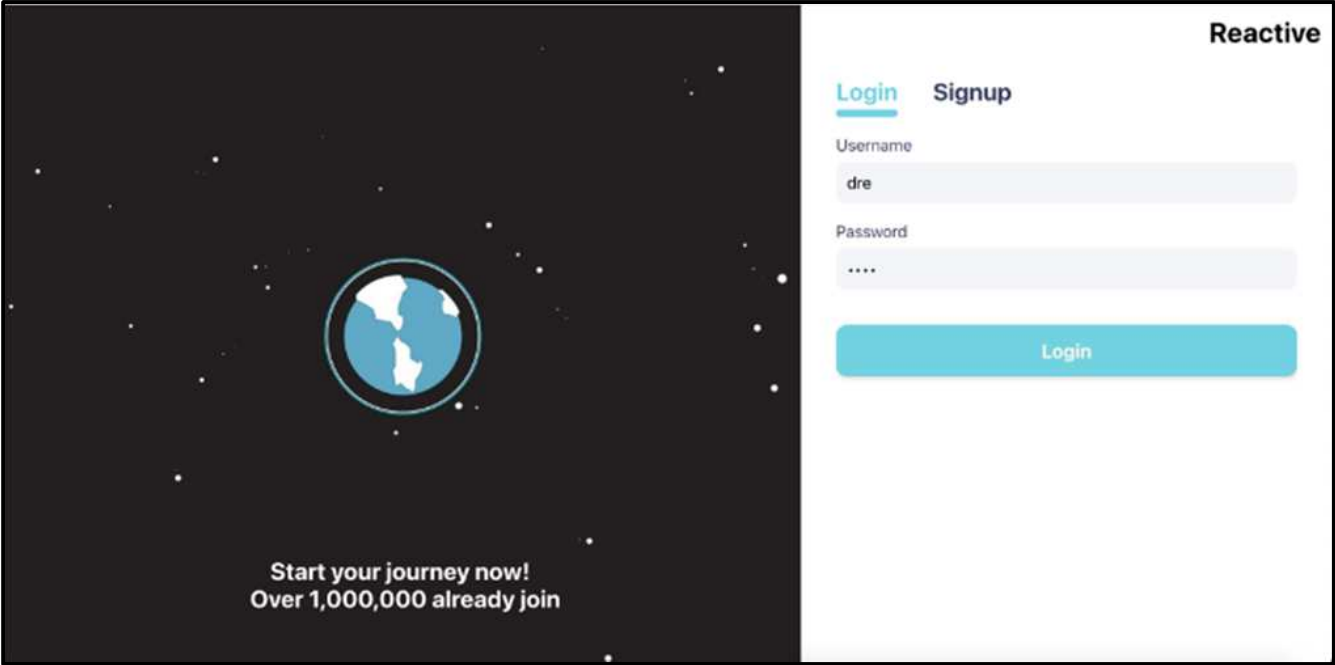
\includegraphics[width=\linewidth]{contents/chapter-2/images/Andre-a1.png}
	  \caption{\textit{Auth Scene}}
	  \label{fig:sub-andre-a1}
	\end{subfigure}
	\begin{subfigure}[b]{0.4\textwidth}
	\centering
	  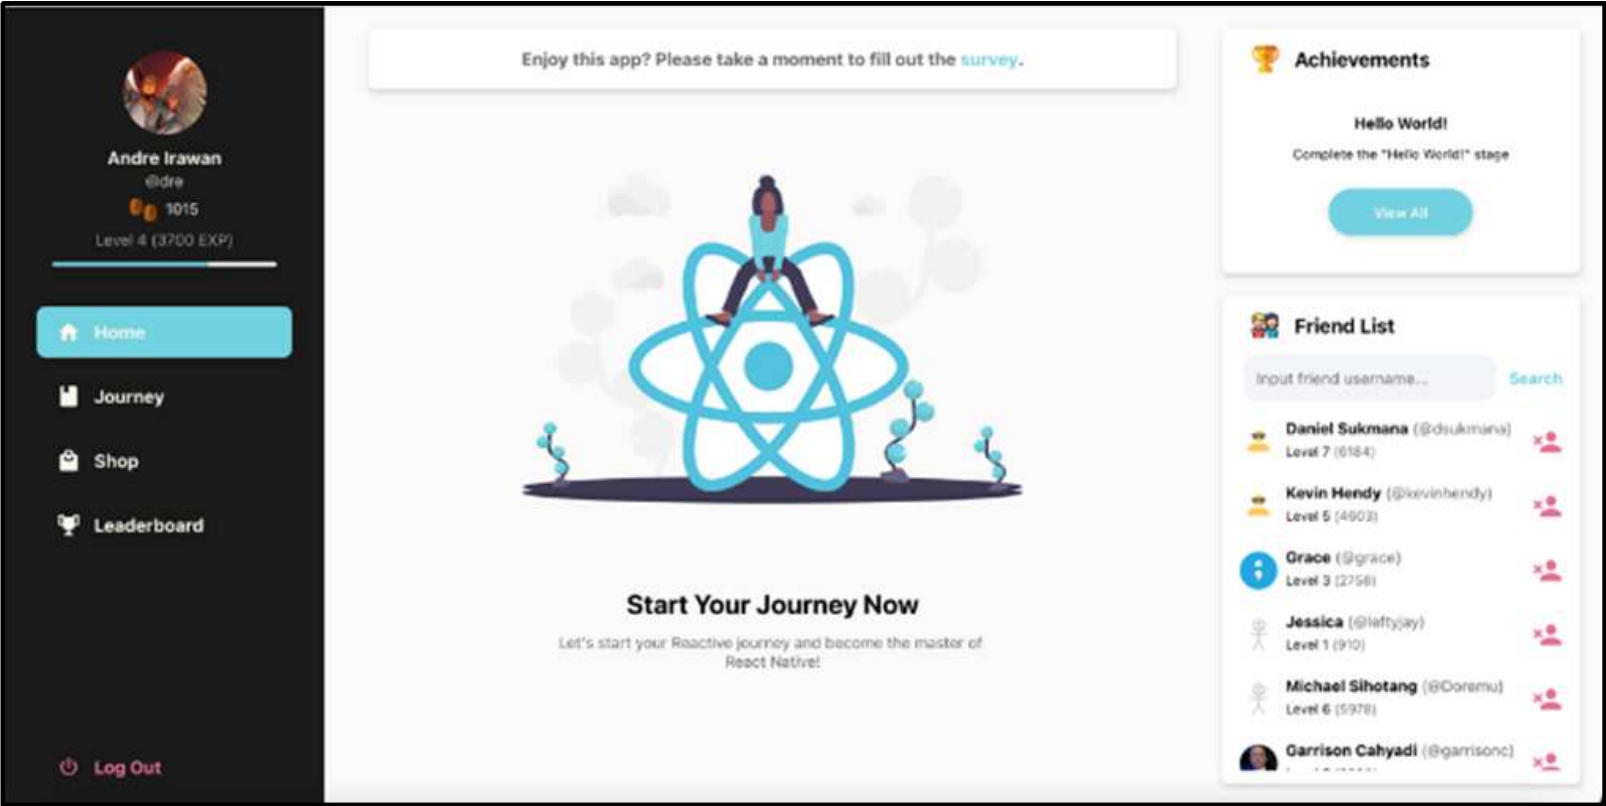
\includegraphics[width=\linewidth]{contents/chapter-2/images/Andre-a3.png}
	  \caption{\textit{Home Scene}}
	  \label{fig:sub-andre-a3}
	\end{subfigure}
	\caption{Tampilam aplikasi pembelajaran \textit{React Native App}\cite{OctalysisFrameworkAndre}}
	\label{fig:interface pembelajaran React Native}
\end{figure}


Untuk mengukur keberhasilan dari penerapan gamifikasi yang dilakukan, penelitian ini mengerjakan beberapa pengujian untuk aplikasi yang dikembangkan.
Penelitian ini menggunakan \textit{Hedonic Motivation System Adoption Model (HMSAM)} untuk mengukur motivasi intrinsik dari sebuah sistem atau aplikasi.
Selain itu juga, dalam penelitian ini dialkukan pengukuran sikap, pendapat, dan persepsi seseorang tentang fenomena sosial dengan skala Likert atau \textit{Likert Scale}\cite{OctalysisFrameworkAndre}.

\begin{figure}[H]
	\centering
	\begin{subfigure}[b]{0.4\textwidth}
		\centering
		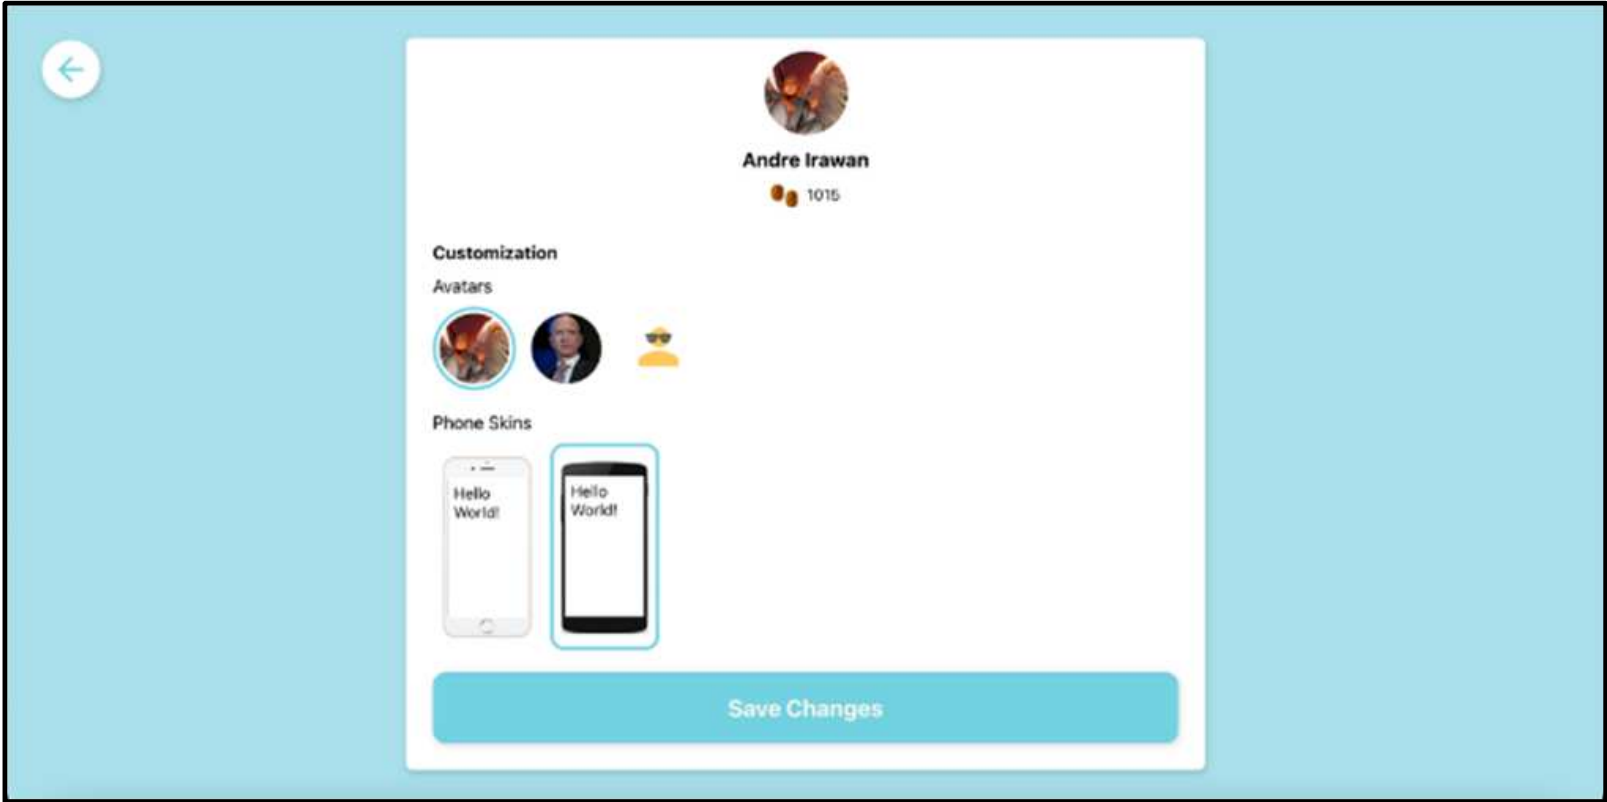
\includegraphics[width=\linewidth]{contents/chapter-2/images/Andre-a4.png}
		\caption{\textit{Edit Profile Scene}}
		\label{fig:sub-andre-a4}
	\end{subfigure}  
	\begin{subfigure}[b]{0.4\textwidth}
		\centering
		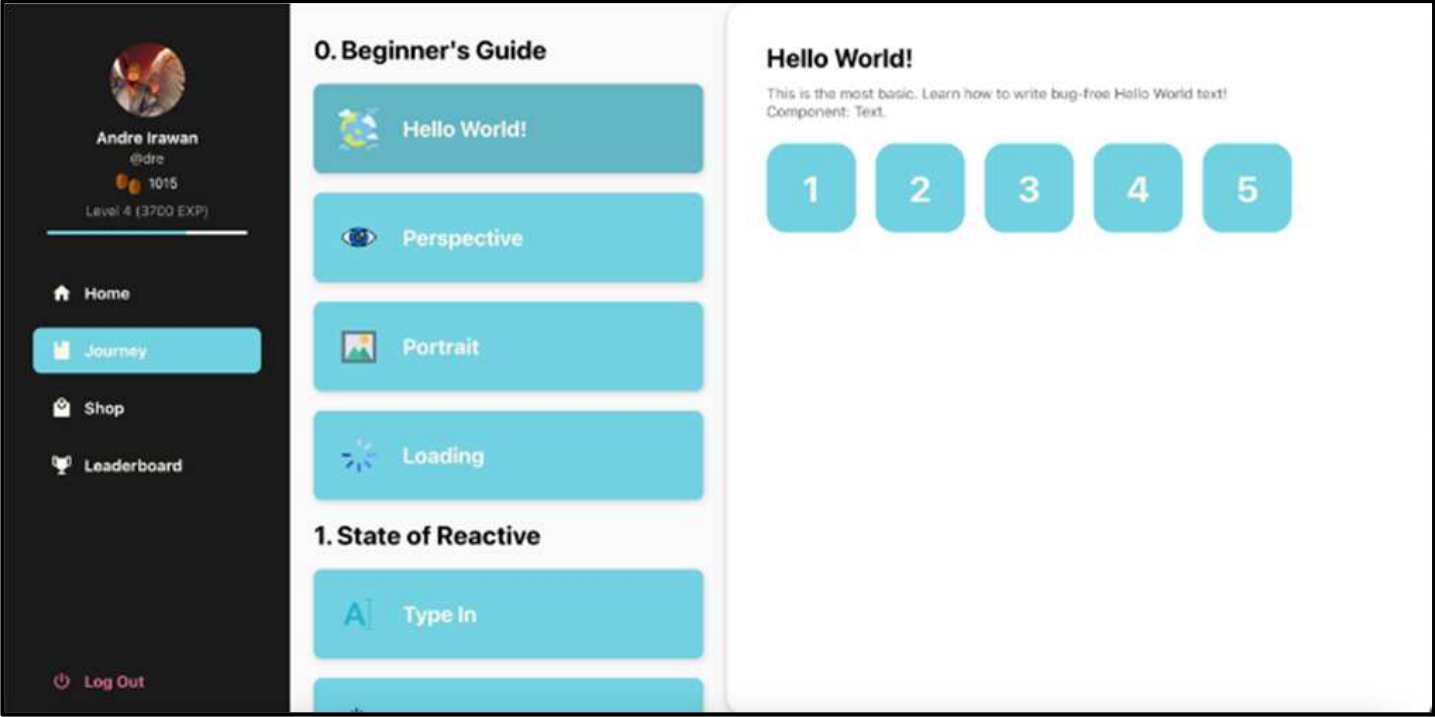
\includegraphics[width=\linewidth]{contents/chapter-2/images/Andre-a5.png}
		\caption{\textit{Journey Module}}
		\label{fig:sub-andre-a5}
	\end{subfigure}
	\hfill
	\begin{subfigure}[b]{0.4\textwidth}
		\centering
		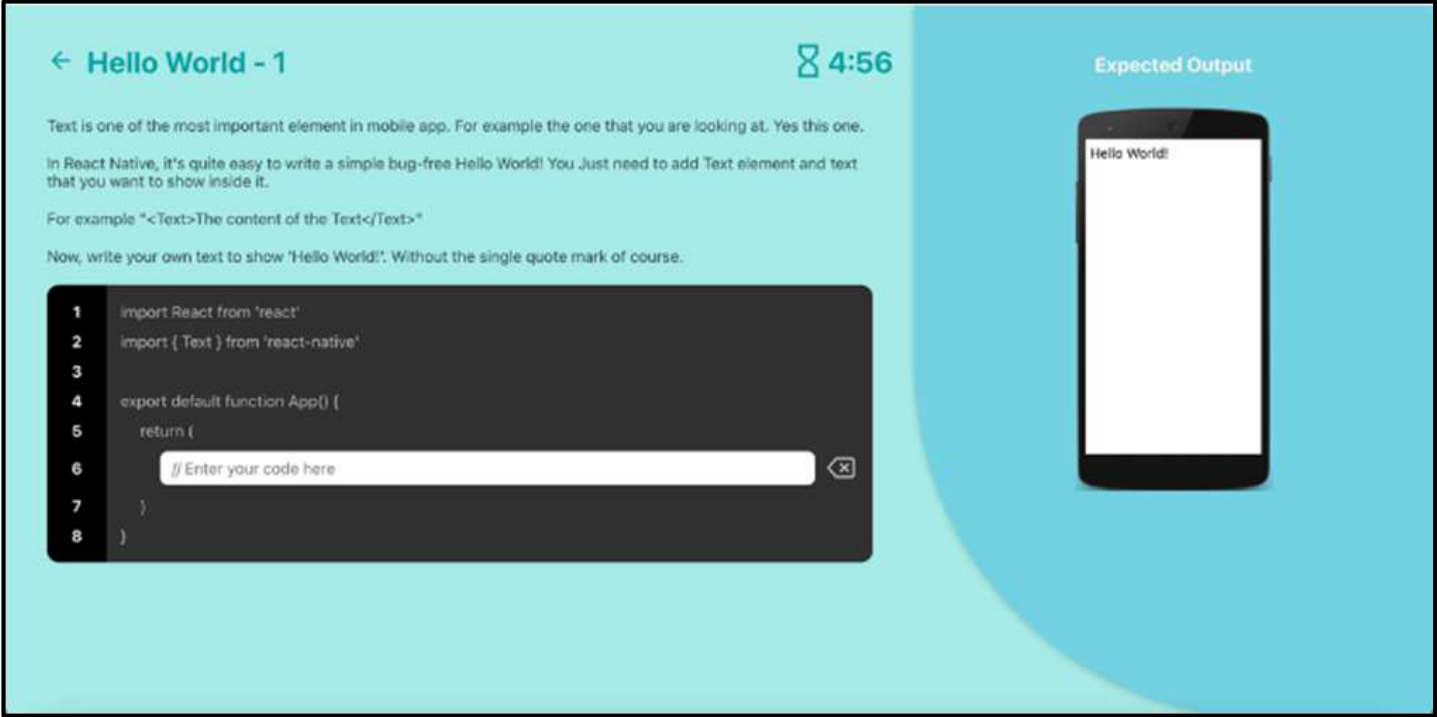
\includegraphics[width=\linewidth]{contents/chapter-2/images/Andre-a6.png}
		\caption{\textit{Level Scene}}
		\label{fig:sub-andre-a6}
	\end{subfigure}
	\begin{subfigure}[b]{0.4\textwidth}
		\centering
		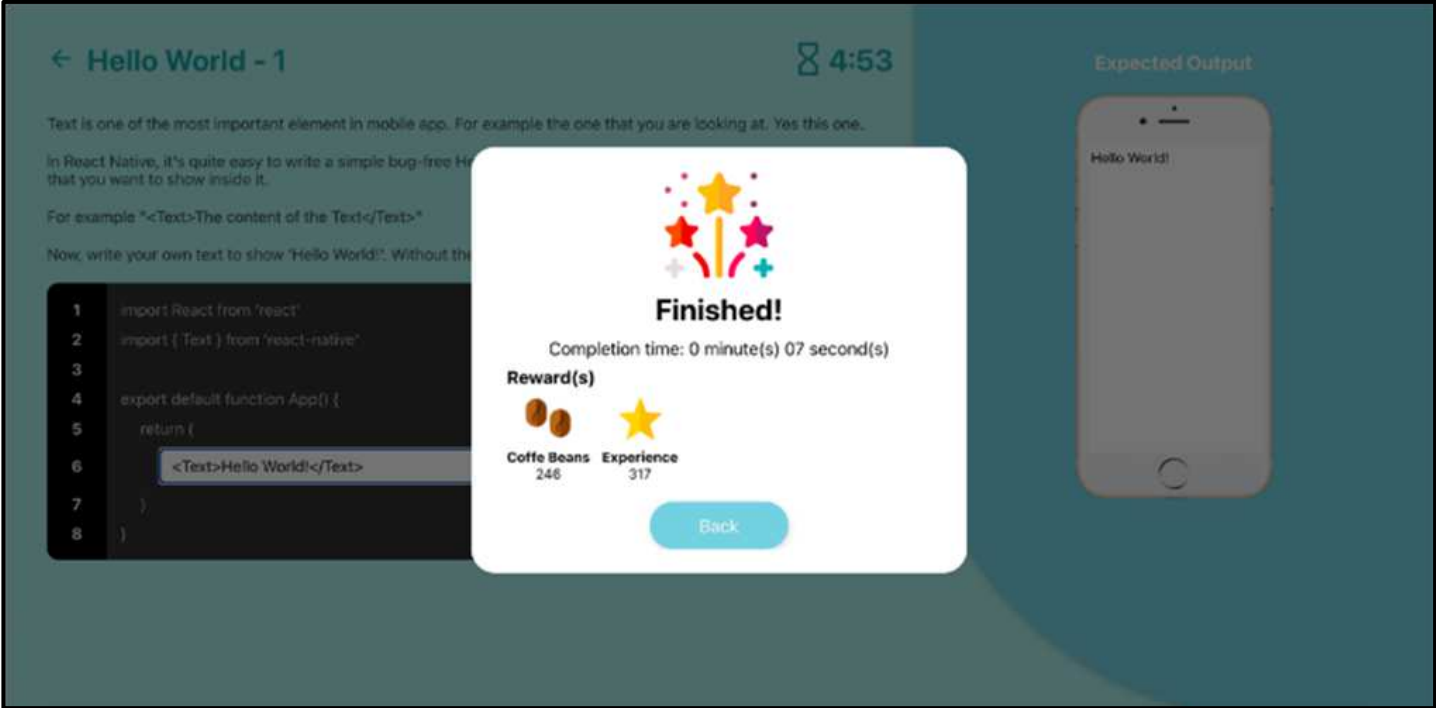
\includegraphics[width=\linewidth]{contents/chapter-2/images/Andre-a7.png}
		\caption{\textit{ Level Scene (Success)}}
		\label{fig:sub-andre-a7}
	\end{subfigure}
	\hfill
	\begin{subfigure}[b]{0.4\textwidth}
		\centering
		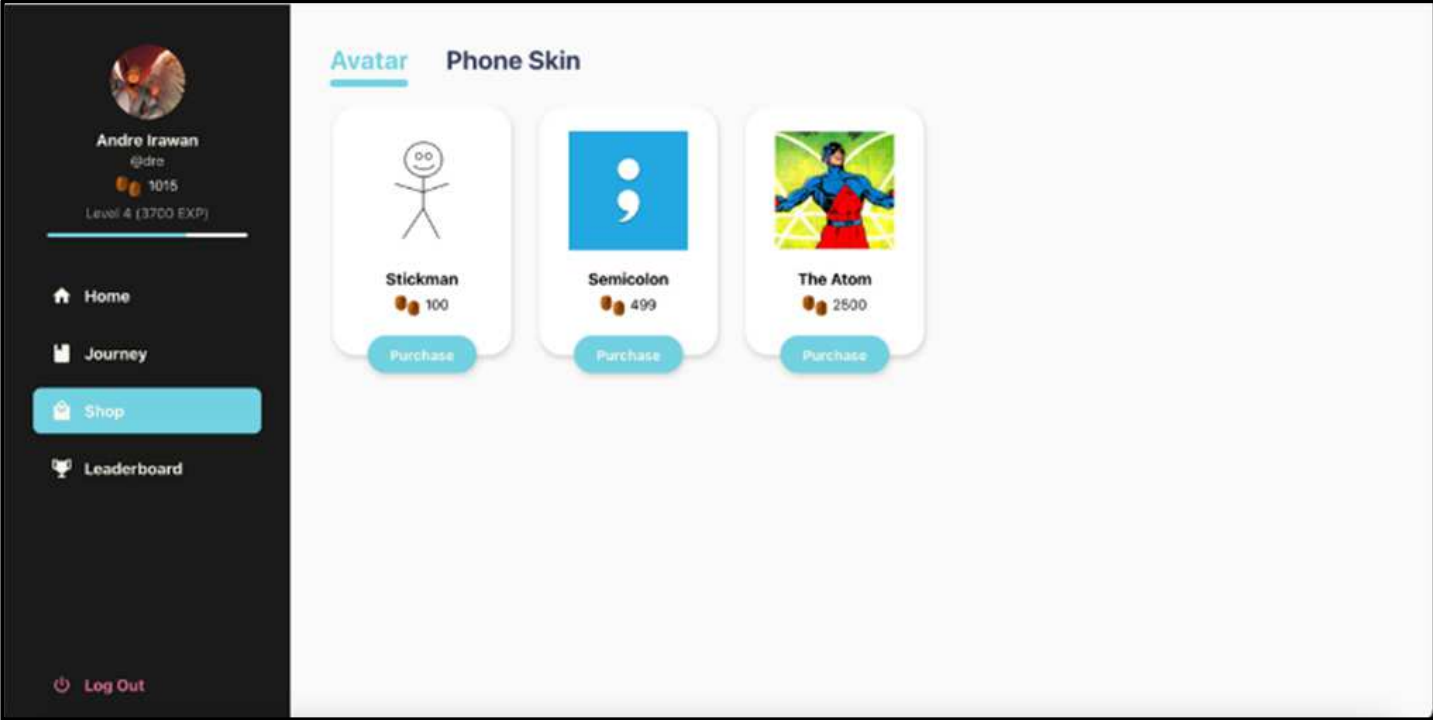
\includegraphics[width=\linewidth]{contents/chapter-2/images/Andre-a8.png}
		\caption{\textit{ Shop Module (Avatar) }}
		\label{fig:sub-andre-a8}
	\end{subfigure}  
	\begin{subfigure}[b]{0.4\textwidth}
		\centering
		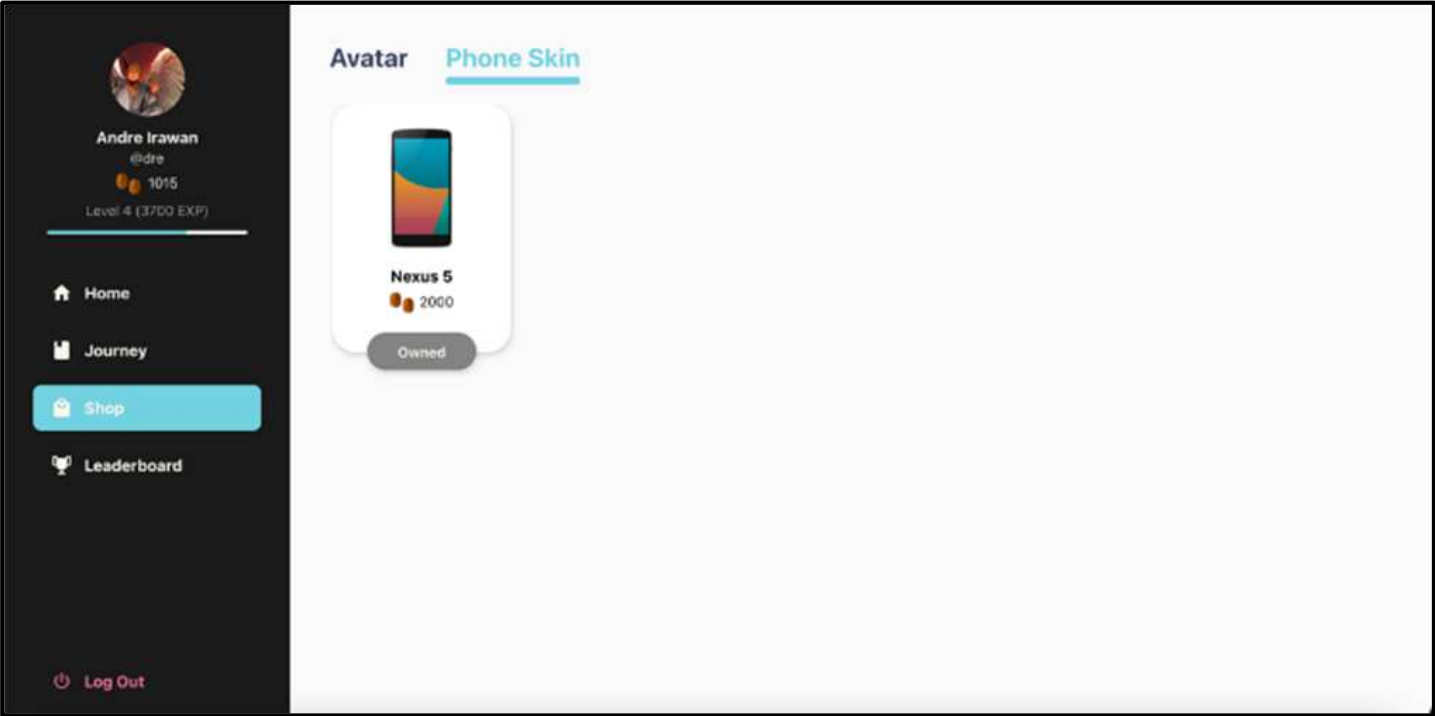
\includegraphics[width=\linewidth]{contents/chapter-2/images/Andre-a9.png}
		\caption{\textit{Shop Module (Phone Skin)}}
		\label{fig:sub-andre-a9}
	\end{subfigure}
	\hfill
	\begin{subfigure}[b]{0.4\textwidth}
		\centering
		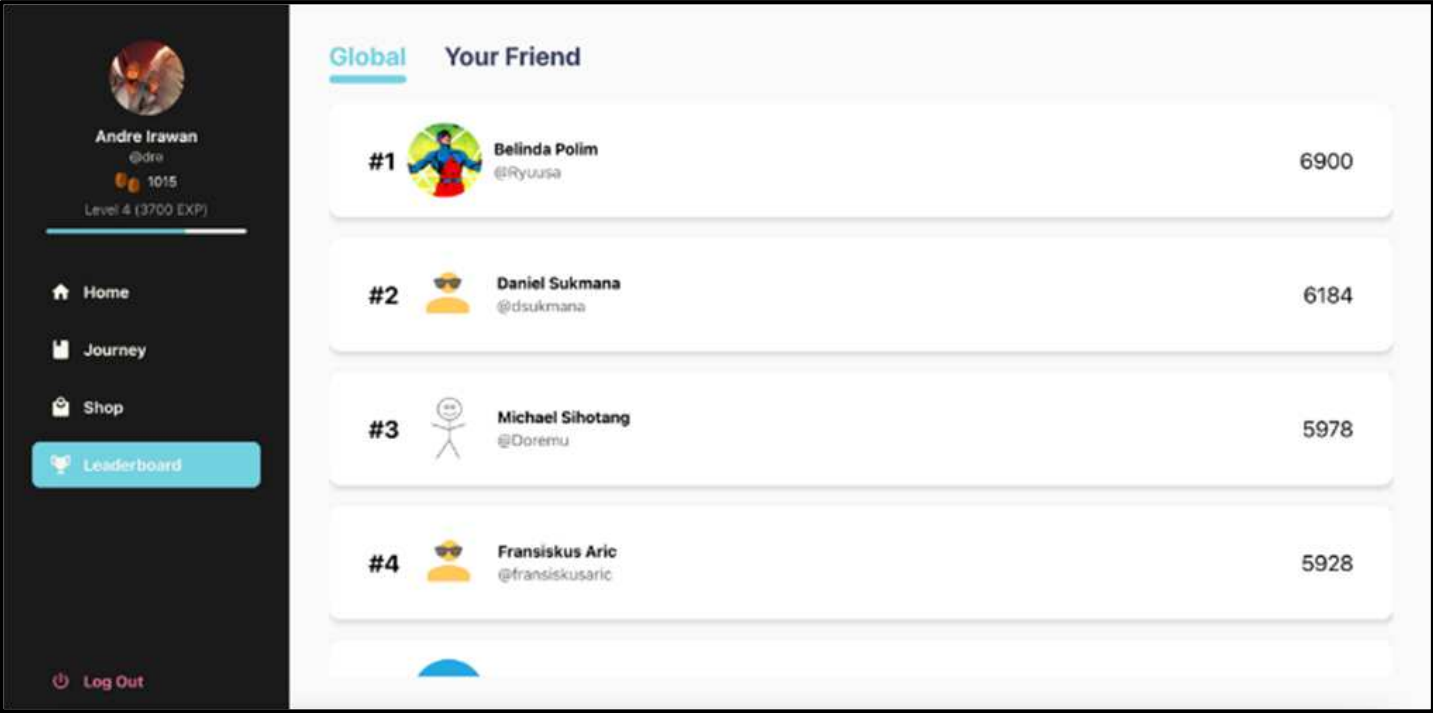
\includegraphics[width=\linewidth]{contents/chapter-2/images/Andre-a10.png}
		\caption{\textit{Leaderboard Module}}
		\label{fig:sub-andre-a10}
	\end{subfigure}
	\caption{Tampilam fitur aplikasi pembelajaran \textit{React Native App}\cite{OctalysisFrameworkAndre}}
	\label{fig:interface fitur pembelajaran React Native}
\end{figure}
Fitur aplikasinya sendiri terdapat pada gambar \ref*{fig:interface fitur pembelajaran React Native}. Fitur yang dikembangkan berupa mengedit \textit{profile} (gambar \ref*{fig:sub-andre-a4}), Memilih modul (gambar \ref*{fig:sub-andre-a5}), Fitur pembalajaran utama yang dibuat berdasarkan level (gambar \ref*{fig:sub-andre-a6}),
fitur menyelesaikan level (gambar \ref*{fig:sub-andre-a7}), Fitur shop (gambar\ref*{fig:sub-andre-a8} dan gambar \ref*{fig:sub-andre-a10}), dan \textit{Leaderboard} (gambar \ref*{fig:sub-andre-a10}) \cite{OctalysisFrameworkAndre}.
\section{Analisis Perbandingan Metode}
Dari tinjauan pustaka yang dilakukan oleh penulis, penulis menemukan perbedaan metode desain dan pengembangan gamifikasi yang digunakan pada setiap penelitian.
Perbedaan ini didasari dengan konteks pembelajaran yang akan dikembangkan, dan bagaimana aplikasi pembelajaran didesain dan dikembangkan.
Faktor lain perbedaan metode ini juga didasari oleh kebutuhan pengguna dan target device dimana aplikasi tersebut akan berjalan.
Penelitian yang dilakukan oleh Evan dan rekan-rekannya menggunakan metode \textit{Activity-centered Design} dimana metode ini dipilih karena aplikasi ini akan berfokus pada aktifitas utama pemrograman.
Berbeda halnya dengan penelitian yang dilakukan oleh Bernadeta dan rekan-rekannya. Metode pengembangan aplikasi ini didasari dengan framework gamifikasi yang diambil dari framework \textit{game design} yang disebut\textit{Elemental Tetrad}.
Penelitian ini mendesain sebuah gamifikasi pembelajaran anatomi berdasarkan setiap elemen yang ada di \textit{Elemental Tetrad Framework}.
Penelitian yang dilakukan oleh Julian dan teman-temannya memiliki metode desain yang sama menggunakan sebuah kerangka kerja gamifikasi, 
bedanya  pada penelitiannya tersebut mereka menggunakan \textit{Octalysis} sebagai kerangka kerjanya. \textit{Framework} ini menggunakan 8 elemen yang fokus pada kebiasaan manusia.
Perbedaan antara kedua \textit{Framework} gamifikasi tersebut adalah dari tujuan kerangka kerjanya. Kerangka kerja \textit{Elemental Tetrad} berfokus pada pembentukan pengalaman Gamifikasi,
sedangkan \textit{Octalysis} berfokus pada pengaruh motivasi dan keterlibatan pengguna dalam gamifikasi. Perbadingan metode dapat dilihat dalam tabel \ref*{Tab: Tabel perbandingan metode}.
Dengan mengadopsi metode-metode yang telah dibahas pada sub bab 2.1, penelitian ini pada dasarnya ialah mencoba untuk meningkatkan kualitas dari sebuah pembelajaran.
Metode pengembangan \textit{Activity-centered Design} yang dilakukan pada penelitian \textit{"Designing Gamification for Programming Learning Applications"} dapat digunakan guna mengembangkan sebuah antar muka yang sesuai dengan tujuan pembelajaran itu sendiri.
Dalam pengembangannya, \textit{framework} gamifikasi dapat diadopsi guna meningkatkan \textit{"Entertainment"}. 
\newpage
\begin{landscape}
	\begin{table}[htbp]
	\caption{Perbandingan Penelitian}
	\centering
	\begin{tabular}{|>{\centering\arraybackslash}m{0.5cm}|m{4cm}|m{3.5cm}|m{4.5cm}|m{4.5cm}|m{4cm}|m{4cm}|}
		\hline
		\centering \textbf{No} & \centering \textbf{Judul Penelitian} & \centering \textbf{Penulis} & \centering  \textbf{Pengembangan Desain Gamifikasi} &\centering\textbf{Fokus}&\multicolumn{1}{m{4cm}|}{\centering\textbf{Luaran}} \\
		\hline 
		1 & "\textit{Designing Gamification for Programming Learning Applications}"
		& 
		Evan Pradanika, Yani Widyani,  Yanti Rusmawati
		& \textit{Activity-centered Design} \& \textit{Type of Knowledge and Gamification Element Relation}& Merancang pengalaman pengguna yang optimal dengan memahami kebutuhan, konteks, dan tujuan aktivitas& \textit{High-fidelity Prototype} Aplikasi\\
		\hline
		2 &"\textit{Design of Gamification for Anatomy Learning Media}" 
		& 
		Adhistya Erna Permanasari, Bernadeta Ratna P S, Fikry Yanuar S, Mirza Putri Maharani, Sunu Wibirama, Junaedy Yunus
		& \textit{Elemental Tetrad Gamification Framework} & Membentuk pengalaman gamifikasi & Aplikasi Mobile\\
		\hline
		3 & 
		"\textit{Implementation of Gamification Octalysis Method at Design and Build a React Native Framework Learning Application}" 
		& 
		Andre Julian Irawan, Fenina Adline Twince Tobing, Eunike Endariahna Surbakti
		& \textit{Octalysis Gamification Framework}& Mempengaruhi Motivasi dan Keterlibatan pengguna & Aplikasi Web \textit{React Native}\\
		\hline
	  \end{tabular}
	  \label{Tab: Tabel perbandingan metode}
	\end{table}
\end{landscape}

\newpage
\section{Dasar Teori}
\subsection{\textit{Clinical Decision Support System}(CDSS)}
\textit{Clinical Decision Support System} atau Sistem pendukung keputusan klinis merupakan sebuah sistem komputer yang dirancang untuk mempengaruhi pengambilan keputusan klinis mengenai pasien individu pada saat keputusan tersebut diambil\cite{sutton2020overview}.
Ilmu ini merupakan kombinasi antara ilmu medis dan ilmu informatika, dimana kita melakukan perhitungan komputasi mengenai sebuah keputusan medis berdasarkan rekam medis individu.
\subsection{Media Pembelajaran}
Secara deskriptif, media pembelajaran merupakan sebuah medium yang memuat informasi atau pesan instruksional yang digunakan dalam proses pembelajaran\cite{hasan2021media}. 
Menurut \textit{Education Association} (NEA) media pembelajaran sebagai benda yang dapat dimanipulasi, dilihat, didengar, dibaca atau dibicarakan 
beserta instrumen yang dipergunakan dengan baik dalam kegiatan belajar mengajar, dapat mempengaruhi efektifitas program instruksional\cite{arsyad2011media}.
Media ini menjadi salah satu instrumen yang strategis dalam penentuan keberhasilan proses belajar mengajar, dan tentu saja sangat penting untuk membantu peserta didik memperoleh konsep baru, keterampilan dan kompetensi \cite{hasan2021media}.
Ada banyak jenis media pembelajaran yang dapat diimplementasikan ke dalam sebuah pembelajaran, namun pemilihan media yang tepat akan berpengaruh pada hasil dari pembelajaran.
\subsubsection{Media Pembelajaran Elektronik}
Media Pembelajaran Elektronik atau yang lebih kita kenal sebagai \textit{E-Learning} merupakan sebuah media pembelajaran modern yang mengadopsi Teknologi Informasi untuk mempermudah penyampaian informasi.
Secara deskriptif, \textit{E-Learning} atau \textit{"Electronic learning} merupakan proses belajar dan mengajar degan menggunakan teknologi elektronik dan internet sebagai media pengirim dan penerima informasi \cite{hanum2013keefetifan}.
Melalui media ini pengguna akan menggunakan perangkat elektronik seperti komputer, laptop, atau smartphone yang dapat mengakses internet untuk mengakses materi pembelajaran, berinteraksi dengan instruktur atau sesama peserta, dan menyelesaikan tugas-tugas atau ujian secara online.
\subsection{Gamifikasi}
Gamifikasi merupakan sebuah pendekatan yang mengadopsi elemen-elemen \textit{game} untuk menyelesaikan masalah non \textit{game} \cite{marisa2020gamifikasi}.
Konsep ini dapat berupa produk, cara berpikir, proses, pengalaman, cara desain, dan sistem dimana intinya ialah menggunakan elemen \textit{game} untuk menyelesaikan masalah non \textit{game}. 
Konsep gamifikasi tentu saja muncul dari karakteristik sebuah \textit{game entertainment} atau permainan yang secara harfiah dibuat untuk menghibur dan dapat menarik pengguna untuk mengoperasikannya.
Seiring perkembangan jaman, \textit{game entertainment} berkembag ke ranah yang lain seperti edukasi yang bertujuan untuk menarik pengguna untuk memotivasi pengguana.
Dengan demikian, konsep \textit{gamifikasi} ditemukan dan dapat diadopsi untuk menyelesaikan sebuah masalah. Visualisasi dari perkembangan ilmu seputar \textit{game} dapat di lihat pada gambar \ref*{Fig:Ilustrasi perkembangan ilmu game}.
\begin{figure}[H]
	\centering
	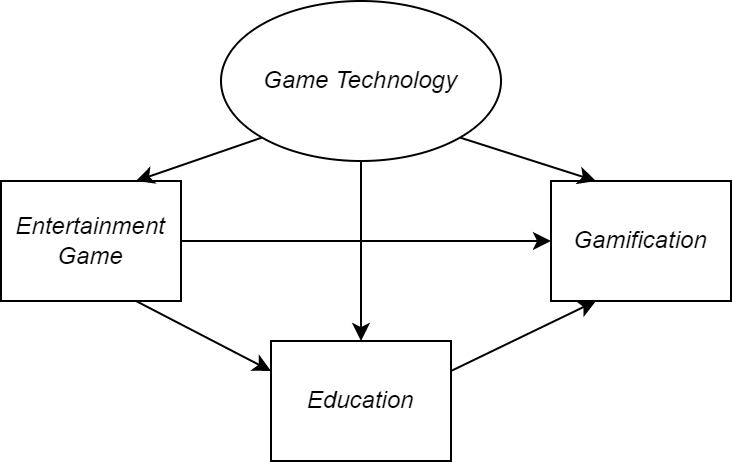
\includegraphics[width=7cm]{contents/chapter-2/images/perkembangan-game.png}
	\caption{Ilustrasi perkembangan ilmu \textit{game} \cite{2004activity}}
	\label{Fig:Ilustrasi perkembangan ilmu game}
\end{figure}
\subsection{Hubungan antara \textit{Type of Knowledge} dan gamifikasinya}
 \begin{table}[H]
	\caption{Domain Pembelajaran dan Teknik Pembelajaran dan Gamifikasi Terkait \cite{kapp2012gamification}}
	\vspace{0.5em}
	\centering
	\begin{tabular}{|m{5cm}|m{5cm}|m{4cm}|}
		\hline
        \multicolumn{1}{|c|}{\textbf{Type of Knowledge}} & \multicolumn{1}{c|}{\textbf{Gamification Elements}} & \multicolumn{1}{c|}{\textbf{Examples}} \\ 
		\hline 
        \hline
		\textit{Declarative Knowledge} & \textit{Stories/Narrative, Sorting, Matching, Replayability} & \textit{Trivia, Hangman, Drag and Drop }\\\hline
		\textit{Conceptual Knowledge} & \textit{Matching and sorting, Experiencing the concept}  & \textit{Wack a Mole, You Bet!} \\\hline
		\textit{Rules-Based Knowledge}  & \textit{Experience Consequences}  & \textit{Board games, Simulated work tasks} \\ \hline
        \textit{Procedural Knowledge } & \textit{Software challenges, Practice} & \textit{Data Miner, Software scenarios} \\\hline
        \textit{Soft Skills} & \textit{Social Simulator}  & \textit{Leadership simulation}  \\\hline
        \textit{Affective Knowledge} & \textit{Immersion, Providing success, Encouragement from a celebrity-type figures } & \textit{Darfur Is Dying}  \\\hline
        \textit{Psychomotor Domain} & \textit{Demonstration, Haptic devices}  & \textit{Virtual Surgery Simulator}  \\
        \hline
	\end{tabular}
	\label{Tab: Tabel Type of Knowledge and Gamification}
\end{table}
\subsection{\textit{Game Thinking}}
\textit{Game thinking} merupakan sebuah pendekatan berpikir yang terinspsirasi oleh prinsip-prinsip desain dan mekanisme permainan dalam konteks non-\textit{game}. 
Ini melibatkan penerapan elemen-elemen permainan, seperti tantangan, imbalan, persaingan, dan pencapaian, dalam lingkungan non-permainan seperti bisnis, pendidikan, atau pengembangan produk\cite{schell2008art}.
Pendekatan ini digunakan dalam proses Gamifikasi untuk menciptakan pengalaman yang lebih menyenangkan, menarik, dan efektif bagi pengguna atau peserta.
\begin{figure}[H]
	\centering
	\begin{subfigure}[b]{0.4\textwidth}
		\centering
	  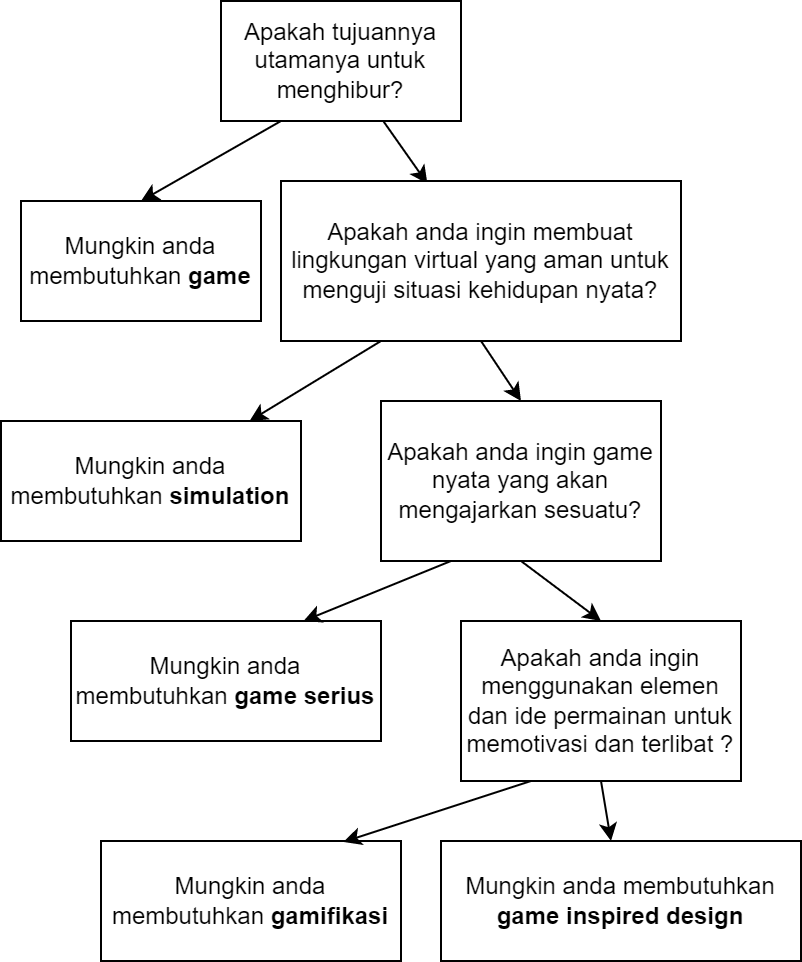
\includegraphics[width=\linewidth]{contents/chapter-2/images/Game-thinking-2.png}
	  \caption{\textit{game thinking}:Apa yang anda butuhkan}
	  \label{fig:sub-gamethink-1}
	\end{subfigure}
	\hfill
	\begin{subfigure}[b]{0.4\textwidth}
	\centering
	  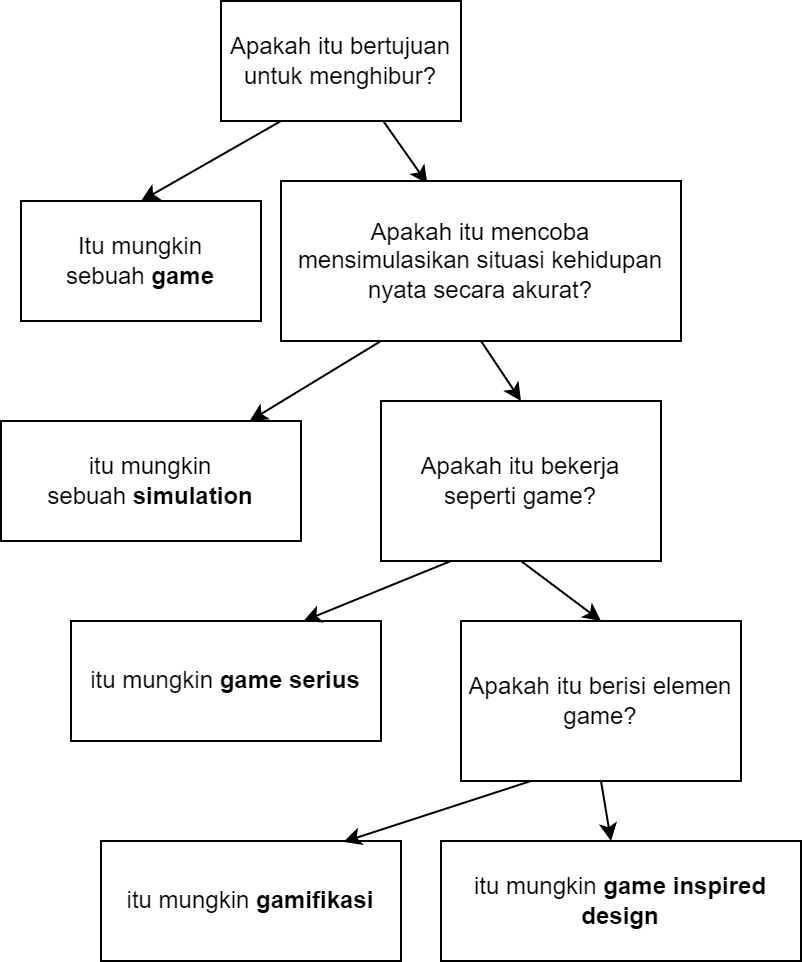
\includegraphics[width=\linewidth]{contents/chapter-2/images/Game-thinking-1.png}
	  \caption{\textit{game thinking}: Apa yang sudah anda dapatkan?}
	  \label{fig:sub-gamethink-2}
	\end{subfigure}
	\caption{\textit{Game Thinking}\cite{marisa2020gamifikasi}}
	\label{fig:Gamethink}
\end{figure}
Dengan konsep tersebut, kerangka kerja gamifikasi dikembangakan dengan tujuan memudahkan pengembangan gamifikasi secara terstruktur dan konsisten.
Kerangka kerja Gamifikasi yang ada saat ini adalah kerangka kerja Octalysis, MDA, Elemental Tetrad, MDE, dan SGD.
\subsubsection{\textit{The MDA Framework}}
MDA \textit{(Mechanics, Dynamics, Aesthetics)} \textit{Framework} adalah sebuah kerangka kerja yang digunakan dalam pengembangan permainan
\textit{(game development)} untuk menganalisis dan memahami elemen-elemen inti yang membentuk pengalaman bermain game \cite{marisa2020gamifikasi}. 
Konsep ini pertama kali diperkenalkan oleh Robin Hunicke, Marc LeBlanc, dan Robert Zubek pada tahun 2004.
Dalam gamifikasi, pendekatan kereangka kerja ini secara formal digunakan dengan menganalisis desain \textit{game} ke dalam 3 elemen,
Ketiga elemen tersebut diantaranya adalah \textit{Mechanics} yang menjelaskan aturan dan komponen permainan tertentu dalam hal tindakan, dan dapat disebut sebagai proses yang mendorong tindakan pengguna.
Kemudian \textit{Dynamics} sebagai elemen yang menguraikan cara implementasi aturan selama permainan \textit{game} berdasarkan tindakan pemain yang diterjemahkan secara langsung ke dalam sistem, serta interaksi yang terjadi antara para pemain.
Lalu, ada juga \textit{Aesthetics} Menjelaskan respons emosional yang diharapkan yang timbul dari pengguna saat berinteraksi dengan sistem yang menggunakan gamifikasi\cite{marisa2020gamifikasi}.
\begin{figure}[H]
	\centering
	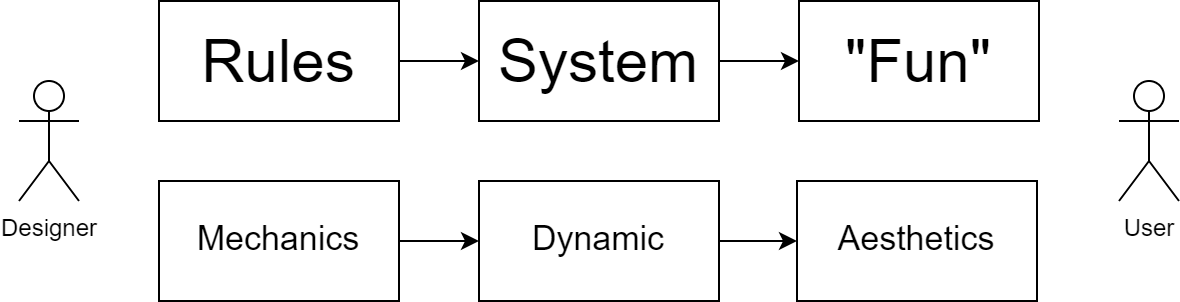
\includegraphics[height=4cm]{contents/chapter-2/images/MDA-framework.png}
	\caption{Ilustrasi \textit{MDA Framework}}
	\label{Fig:Ilustrasi MDA}
\end{figure}
Gambar \ref*{Fig:Ilustrasi MDA} menunjukkan sebuah ilustrasi dari pengembangan gamifiakasi menggunakan kerangka kerja MDA.
Kerangka kerja MDA digambarkan sebagai hubungan satu arah dari desainer ke pengguna.
Kerangka kerja ini memungkinkan desainer membangun fungsi \textit{(Mechanics)} yang pada gilirannya menyediakan interaksi pengguna yang berbeda \textit{(Dynamics)}, yang membawa emosi dan pengalaman kepada pengguna \textit{(Aesthetics)}.
Biasanya, desainer lebih cenderung melihat permainan dari aspek mekanika \textit{(Mechanics)}, kemudian dinamika \textit{(Dynamics)}, dan terakhir estetika \textit{(Aesthetics)}, 
sedangkan pemain cenderung melihat ke arah yang berlawanan dimulai dari aspek estetika \textit{(Aesthetics)}, kemudian dinamika \textit{(Dynamics)}, dan terakhir mekanika \textit{(Dynamics)}.

Mekanika \textit{(Mechanics)} berhubungan dengan elemen-elemen, kontrol, dan aturan yang diimplementasikan dalam permainan, seperti tindakan dasar, algoritma, mesin permainan, unsur-unsur permainan, dan sebagainya.
Mekanika melibatkan berbagai tindakan, algoritma, dan struktur data dalam mesin permainan yang secara keseluruhan mendukung dinamika dalam permainan.
Dinamika \textit{(Dynamics)} menjelaskan bagaimana mekanika dalam permainan bekerja berdasarkan input dari pemain dan hubungannya dengan mekanika lainnya.
Dinamika \textit{(Dynamics)} memiliki potensi untuk menciptakan estetika \textit{(Aesthetics)} bagi siapa pun yang memainkan \textit{game}. Estetika ini dapat berupa kepuasan, kekecewaan, kebimbangan, keragu-raguan, dan berbagai perasaan lainnya yang timbul selama permainan.
\subsection{\textit{Activity-centered Design}}
\textit{Activity-centered Design} atau (ACD) merupakan metode desain sebuah sistem yang berfokus pada perilaku yang berkaitan dengan tugas tertentu.
Pendekatan ini cocok untuk mendesain sebuah sistem yang memerlukan tindakan kompleks dengan pengguna yang beragam. Metode ini menggunakan \textit{Iterative Design Cycle} seperti pada gambar \ref*{Fig:itterative-Design Cycle}.
\begin{figure}[H]
	\centering
	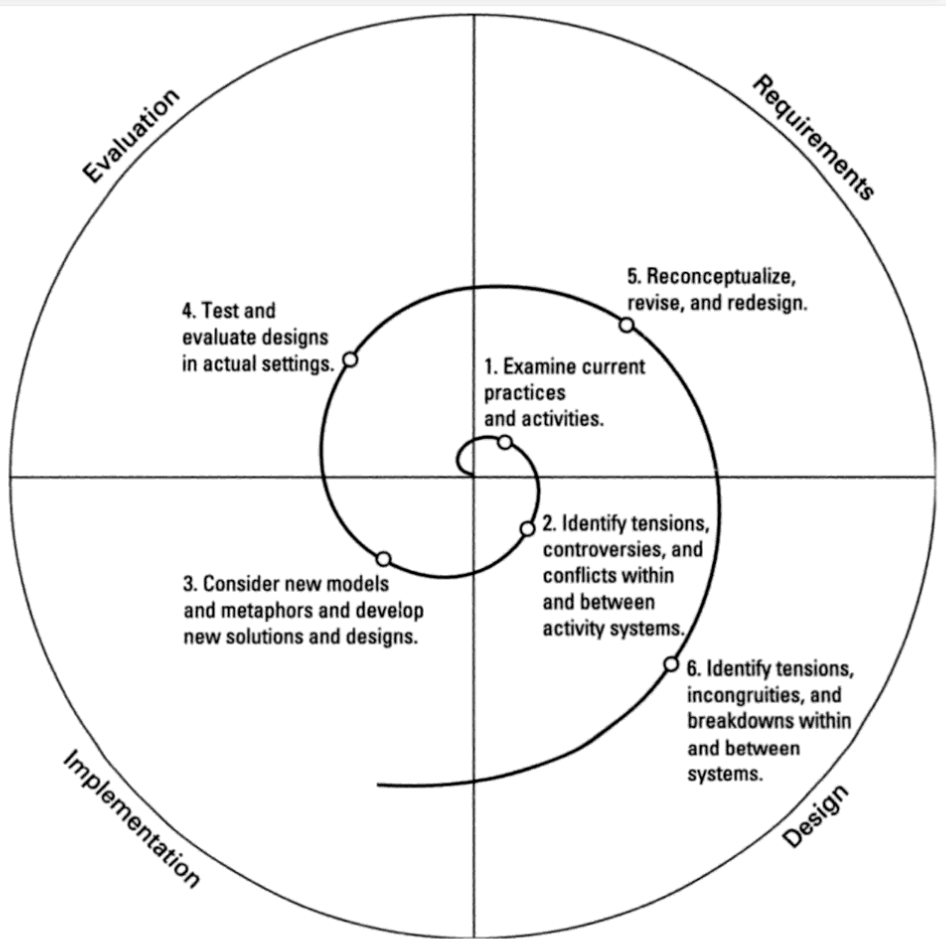
\includegraphics[height=8cm]{contents/chapter-2/images/Itterative-design.png}
	\caption{An itterative-Design Cycle \cite{2004activity}}
	\label{Fig:itterative-Design Cycle}
\end{figure}
Tahap pertama pada metode ini ialah tahap \textit{Requirements}. Pada tahap ini, dilakukan identifikasi kebutuhan dan aktivitas. 
Kemudian pada tahap Desain \textit{Design}, dilakukan identifikasi dan penyelesaian konflik yang mungkin timbul antara aktivitas dalam sistem.
Selanjutnya pada tahap \textit{Implementasi}, solusi dan desain dikembangkan dan dievaluasi pada tahap \textit{Evaluation}.
Akhirnya, siklus tersebut diulang hingga kebutuhan sistem tercapai.
\subsection{\textit{Feature-Driven Development}}
\textit{Feature-Driven Development} (FDD) adalah metode pengembangan perangkat lunak yang mengadopsi pendekatan iteratif dan merupakan salah satu pendekatan dalam kerangka metodologi \textit{Agile}.
Proses pengembangan perangkat lunak ini terdiri dari 5 aktivitas utama, yaitu \textit{Develop Overall Model}, \textit{Plan by Features}, \textit{Design by Features}, dan \textit{Build by Features}.
5 aktivitas tersebut divisualisasikan oleh gambar \ref*{Fig:FDD-langkah}.
\begin{figure}[H]
	\centering
	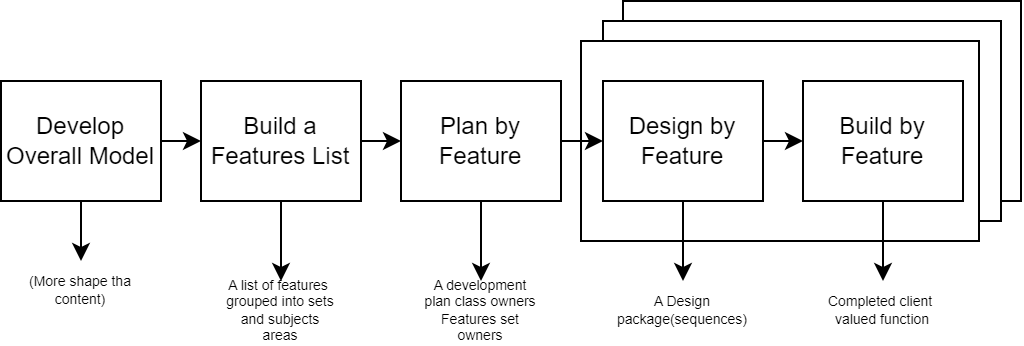
\includegraphics[width=\textwidth]{contents/chapter-2/images/FDD.png}
	\caption{Aktivitas utama \textit{Feature-driven Development}\cite{palmer2001practical}}
	\label{Fig:FDD-langkah}
\end{figure}
Aktivitas yang pertama ialah \textit{Develop Overall Model}, proses ini merupakan proses identifikasi dan memahami dasar permasalahan yang akan ditangani oleh perangkat lunak yang akan dikembangakan.
Hasilnya berupa \textit{high-level object model} yang sepanjang proses pengembangan akan terus disempurnakan. Dilanjutkan dengan proses \textit{Build a Features List} dengan membuat daftar fitur yang akan dikembangkan dan mengelompokkannya ke dalam kelompok atau set terkait.
Kemudian, proses \textit{Plan by Feature} merupakan aktivitas yang menentukan pemilik dari suatu \textit{Class} atau kelompok fitur.
Setelah itu, untuk proses \textit{Design by Feature} dan \textit{Build by Feature} merupakan proses \textit{modeling} yang lebih detail hingga mendapatkan hasil yang sesuai dengan kebutuhan.
Proses \textit{modeling} tersebut termasuk pengembangan kode, dan \textit{Testing system}.
\subsection{\textit{Black Box Testing}}
\textit{Black Box Testing} merupakan salah satu pengujian yang dilakukan pada sebuah perangkat lunak.
Pengujian ini berfokus pada suatu fungsionalitas suatu perangkat lunak, dimana fokus utamanya ialah input yang tersedia untuk suatu sistem dan output yang diharapkan untuk setiap nilai input.
Metode \textit{Black Box Testing} didasari oleh \textit{software requirements} dan \textit{specification}. Ini adalah teknik pengujian perangkat lunak di mana cara kerja internal dari \textit{item} yang diuji tidak diketahui oleh pengujian.
Metode ini juga disebut pengujian berbasis spesifikasi dan perilaku. 
Teknik ini dinamai demikian karena dalam pengujian ini, pengujian tidak perlu mengetahui implementasi kode internal aplikasi\cite{beizer1995black}.
Pengujian ini menangani input valid dan tidak valid sesuai dengan kebutuhan \textit{User}. Representasi pengujian ini divisualisasikan oleh gambar \ref*{Fig:Black Box Testing}.
\begin{figure}[H]
	\centering
	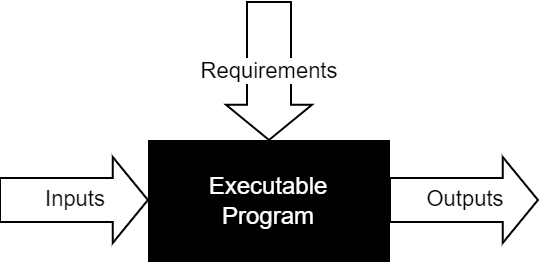
\includegraphics[width=8cm]{contents/chapter-2/images/BlackBox-Testing.png}
	\caption{Representasi \textit{Black Box Testing}\cite{beizer1995black}}
	\label{Fig:Black Box Testing}
\end{figure}
Dalam melakukan pengujian ini, ada beberapa teknik yang dapat dilakukan. Teknik-teknik tersebut diantaranya ialah:
\begin{description}
	\item[\textit{Equivalence partitioning}]teknik ini digunakan untuk merancang kasus uji \textit{(Test Cases)}. Dalam metode ini, nilai-nilai input diambil dan dikelompokkan ke dalam partisi-partisi. Partisi tersebut terdiri dari nilai-nilai yang valid dan tidak valid. Kasus uji kemudian dirancang dari setiap partisi untuk mendeteksi kesalahan yang mungkin terjadi
	\item[\textit{Boundary Value Analysis}]Teknik ini digunakan untuk merancang kasus uji guna mengungkap kesalahan. Dalam teknik ini, diambil nilai batas atau nilai batas terdekat dari domain input sebagai data uji. Kasus Uji dirancang untuk nilai batas yang valid maupun tidak valid. Satu Kasus Uji dipilih dari setiap nilai batas.
	\item[\textit{Cause Effect Graphing}]Ini adalah teknik perancangan pengujian perangkat lunak yang berfokus pada perilaku eksternal sistem. Teknik ini menentukan hubungan logis antara kondisi masukan dan keluaran dengan bantuan operator Boolean. Nilai masukan mewakili 'Penyebab' dan nilai keluaran mewakili 'Efek'. Hubungan antara Penyebab dan Efek membantu dalam membuat kasus uji.
	\item[\textit{Decision Table Based Testing}]Ini adalah teknik yang baik untuk menangani sejumlah besar input dan keluaran yang terkait. Decision Table memiliki sifat kelengkapannya; tabel ini berisi semua kemungkinan nilai dari kondisi yang ada. Ini sangat berguna untuk mengubah alur bisnis yang kompleks menjadi kasus uji.
	\item[\textit{Error Guessing}]Ini adalah teknik untuk mengasumsikan dan menebak. Tester berpengalaman mencari tahu cacat-cacat yang ada. Keberhasilan teknik ini sepenuhnya bergantung pada kemampuan \textit{tester}, seorang \textit{ tester} yang baik tahu di mana dan jenis cacat yang paling sering ditemukan.
\end{description}
% Setiap pengujian perangkat lunak tentu saja memiliki kelebihan dan kekurangannya masing masing.
% Pengujian \textit{Black Box Testing} sendiri memiliki keuntungan sebagai berikut:
% \begin{enumerate}
% 	\item Pengujian dilakukan sesuai dengan kebutuhan pandangan pengguna.
% 	\item Pengujian dilakukan oleh pihak ketiga untuk menghindari bias pengembang.
% 	\item Tester dapat berupa orang non-teknis. Pengetahuan tentang pemrograman dan implementasi tidak diperlukan untuk teknik pengujian ini.
% 	\item Pengujian ini efisien ketika digunakan pada sistem yang lebih besar. Kasus uji dapat dirancang segera setelah spesifikasi selesai.
% \end{enumerate} 
% Ada juga kekurangan yang mungkin terjadi pada pengujian Ini

\subsection{\textit{System Usability Scale}(SUS)}
Pengujian kebergunaan atau \textit{Usability Testing} merupakan salah satu upaya proses evaluasi yang dilakukan untuk mengukur sejauh mana sebuah produk atau sistem memenuhi kebutuhan dan harapan pengguna\cite{dumas1999practical}. 
Tujuan dari pengujian kebergunaan adalah untuk memastikan bahwa produk atau sistem dapat digunakan dengan mudah, efektif, dan memuaskan pengguna.
Salah satu cara untuk mengukur kebergunaan adalah dengan menggunakan \textit{System Usability Scale}. \textit{System Usability Scale} atau (SUS) merupakan sebuah kuesioner yang digunakan untuk mengukur tingkat kegunaan dari suatu sistem berdasar sudut pandang subjektif pengguna.
Hasil pengujian SUS adalah skor dengan rentang nilai 1-100 dan tidak menggunakan perhitungan yang rumit. 
Kuesioner SUS terdiri dari sepuluh pertanyaan yang mengandung pernyataan positif dan negatif\cite{dumas1999practical}. 
Responden diminta untuk memberikan jawaban berdasarkan skala 1-5, di mana 1 menunjukkan "Sangat Tidak Setuju", 2 menunjukkan "Tidak Setuju", 3 menunjukkan "Netral", 4 menunjukkan "Setuju", dan 5 menunjukkan "Sangat Setuju".
\begin{table}[H]
	\caption{Tabel pertanyaan kuesioner}
	\label{Tabel pertanyaan kuesioner sus}
	\centering
	\begin{tabular}{|c|m{7cm}|m{0.5cm}|m{0.5cm}|m{0.5cm}|m{0.5cm}|m{0.5cm}|}
		\hline
		\multirow{2}{1cm}{Kode} & \multirow{2}{7cm}{\centering Pertanyaan}& \multicolumn{5}{c|}{\centering Jawaban} \\
		\cline{3-7}
		 & &\centering 1 & \centering  2 & \centering 3 & \centering 4 & \multicolumn{1}{m{0.5cm}|}{\centering 5} \\
		 \hline
		 Q1&Menurut saya, saya akan sering menggunakan aplikasi ini& &  &  &  &  \\
		 \hline
		 Q2&Menurut saya aplikasi ini cukup rumit& & & &  &  \\
		 \hline
		 Q3&Menurut saya aplikasi ini mudah digunakan& & & & & \\
		 \hline
		 Q4&Menurut saya, saya perlu bantuan orang teknis agar dapat menggunakan sistem ini& & & & & \\
		 \hline
		 Q5&Menurut saya, fungsi-fungsi dalam aplikasi ini sudah terintegrasi dengan baik& & & & & \\
		 \hline
		 Q6&Menurut saya, banyak fitur aplikasi yang tidak konsisten& & & & & \\
		 \hline
		 Q7&Menurut saya, aplikasi ini akan cepat dipelajari oleh banyak orang& & & & & \\
		 \hline
		 Q8&Menurut saya aplikasi ini susah digunakan& & & & & \\
		 \hline
		 Q9&Saya merasa percaya diri ketika menggunakan aplikasi ini& & & & & \\
		 \hline
		 Q10&Saya harus mempelajari banyak hal agar dapat menggunakan aplikasi ini& & & & & \\
		 \hline
	\end{tabular}
\end{table}
Setiap pertanyaan memiliki skor kontribusi antara 0 hingga 4. 
Untuk pertanyaan positif dengan angka ganjil (1, 3, 5, 7, dan 9), skor kontribusi diperoleh dengan mengurangi 1 dari posisi skala.
Sedangkan untuk pertanyaan negatif dengan angka genap (2, 4, 6, 8, dan 10), skor kontribusi diperoleh dengan mengurangi posisi skala dari 5.
Selanjutnya, nilai kontribusi total dari setiap pertanyaan dikalikan dengan 2,5 untuk mendapatkan skor akhir dari SUS. Berikut adalah rumus untuk menghitung skor SUS bagi setiap responden.
\begin{equation}
\begin{split}
	\text{SUS Score} = ((Q1-1)+(5-Q2)+(Q3-1)+(5-Q4)+(Q5-1)+ \\ 
	(5-Q6)+(Q7-1)+(5-Q8)+(Q9-1)+(5-Q10))*2.5
\end{split}
\end{equation}
Skor akhir SUS didapatkan dari perhitungan rata-rata skor SUS dari setiap responden.
Menurut studi yang dilakukan oleh Bangor et al., 
jika rata-rata skor SUS berada di bawah 20,3, maka dikategorikan sebagai \textit{"Worst"}.
Jika rata-rata skor berada di atas 20,3, maka dikategorikan sebagai\textit{ "Awful"}. 
Rata-rata skor di atas 35,7 dikategorikan sebagai \textit{"Poor"}, di atas 50,9 sebagai \textit{"OK"}, di atas 71,4 sebagai \textit{"Good"}, di atas 85,5 sebagai \textit{"Excellent"}, dan di atas 90,9 sebagai \textit{"Best"}.
\begin{equation}
	\begin{split}
		\text{SUS Average} = \frac{\sum \text{(SUS Score Individual)}}{\text{Total respondents}} 
	\end{split}
	\label{Perhitungan rata-rata skor SUS}
\end{equation}
\begin{table}[htbp]
	\centering
	\caption{Kategori rata rata hasik skor \textit{SUS}}
	\begin{tabular}{|m{0.1\textwidth}|m{0.1\textwidth}|m{0.1\textwidth}|m{0.1\textwidth}|m{0.1\textwidth}|m{0.1\textwidth}|m{0.1\textwidth}|}
		\hline
		Worst & Awful & Poor & Ok & good & Excellent & Best \\
		\hline
		< 20,3 & >20,3 & >35,7& >50,9 & >71,4& >85,5 & >90,9 \\
		\hline
	\end{tabular}
\end{table}

\subsection{\textit{User Experience Questionnaire}(UEQ)}
\textit{User Experience Questionnaire (UEQ)} adalah sebuah kuesioner yang digunakan untuk mengukur pengalaman pengguna dari suatu produk interaktif.
Kuesioner ini merupakan alat yang sering digunakan untuk mengevaluasi kualitas dan kegunaan perangkat lunak berdasarkan pendapat pengguna. 
Kuesioner UEQ pertama kali dibuat dalam versi bahasa Jerman oleh Schrepp et al. pada tahun 2005.
Saat ini, kuesioner UEQ telah diterjemahkan ke dalam 20 bahasa. Kuesioner UEQ adalah metode pengukuran yang mudah digunakan, dapat diandalkan, dan valid untuk mengukur pengalaman pengguna.
Kuesioner ini dapat digunakan sebagai tambahan dalam metode evaluasi lain untuk mendapatkan penilaian kualitas subjektif.

Evaluasi pengukuran berbasis kuesioner UEQ dibagi menjadi 6 skala aspek 
dengan 26 butir pernyataan , yaitu :
\begin{enumerate}
	\item \textit{Attractiveness}: Seberapa menarik suatu produk secara keseluruhan 
	\item \textit{Perspicuity}:  Seberapa mudah suatu produk digunakan oleh pengguna 
	\item \textit{Efficiency}: Seberapa cepat pengguna menyelesaikan tugas pada suatu produk tanpa kesusahan 
	\item \textit{Dependability}: Seberapa besar kontrol pengguna dalam menggunakan produk  
	\item \textit{Stimulation}: Seberapa baik suatu produk memotivasi pengguna 
	\item \textit{Novelty}: Seberapa inovatif dan kreatif suatu produk 
\end{enumerate}
Skala keattraktifan terdiri dari enam pernyataan, sementara skala aspek lainnya terdiri dari empat pernyataan. Setiap pernyataan memiliki tujuh rentang skala dari -3 hingga +3. Rentang -3 menggambarkan jawaban yang paling negatif, 0 menggambarkan jawaban netral, dan +3 menggambarkan jawaban yang paling positif.
Setelah mengumpulkan hasil kuesioner UEQ, langkah selanjutnya adalah menganalisis data kuesioner tersebut untuk mendapatkan ukuran kinerja dari produk yang dievaluasi. Hasil evaluasi kuesioner UEQ terhadap suatu produk dikelompokkan ke dalam lima kategori berdasarkan skala aspek yang diukur.

\begin{enumerate}
	\item \textit{Excellent}: berada dalam 10\% hasil terbaik.
	\item \textit{Good}: 10\% hasil dalam kumpulan data tolak ukur lebih baik dan 75\% hasil lainnya lebih buruk. 
	\item \textit{Above Average}: 25\% hasil dalam kumpulan data tolak ukur lebih baik dan 50\% hasil lainnya lebih buruk 
	\item \textit{Below Average}: 50\% hasil dalam kumpulan data tolak ukur lebih baik dan 25\% hasil lainnya lebih buruk. 
	\item \textit{ Bad}: berada dalam 25\% hasil paling buruk. 
\end{enumerate}
\begin{figure}[H]
	\centering
	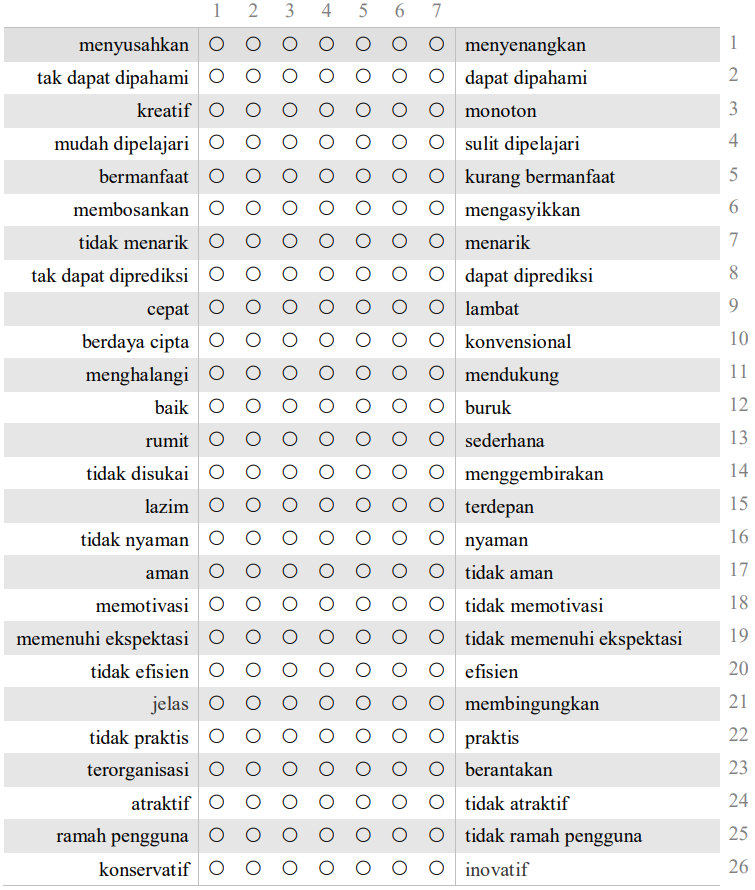
\includegraphics[width=8cm]{contents/chapter-2/images/UEQ-1.png}
	\caption{Pertanyaan kuesioner \textit{User Experience Questionnaire}(UEQ)}
	\label{Fig:UEQ}
\end{figure}
% Di dalam tinjauan pustaka hasil akhirnya adalah analisis secara kualitatif atau pun secara kuantitatif kelebihan dan kekurangan metode jika dikaitkan dengan masalah, batasan-batasan masalah dan solusi yang dinginkan.
% Analisis kuantitatif tidak wajib teapi mempunyai nilai tambah di dalam tugas akhir saudara. Bagian ini menjelaskan kenapa metode tersebut dipilih dan uraikan dengan lebih jelas metode pelaksanaan tugas akhir yang ingin Anda lakukan. 
% \section{Pertanyaan Tugas Akhir (Jika Perlu)}

% Pertanyaan tugas akhir bersifat opsional dan dapat ditambahkan untuk menekankan hal-hal yang hendak diketahui dari tugas akhir berdasar pada tujuan tugas akhir. Pertanyaan tugas akhir dikenal dengan RQ (\textit{Research Question}) dan harus memiliki keterkaitan dengan RO (\textit{Research Objective}). Satu RO dapat memiliki satu atau lebih dari satu RQ. 

